\documentclass[twoside]{book}

% Packages required by doxygen
\usepackage{fixltx2e}
\usepackage{calc}
\usepackage{doxygen}
\usepackage[export]{adjustbox} % also loads graphicx
\usepackage{graphicx}
\usepackage[utf8]{inputenc}
\usepackage{makeidx}
\usepackage{multicol}
\usepackage{multirow}
\PassOptionsToPackage{warn}{textcomp}
\usepackage{textcomp}
\usepackage[nointegrals]{wasysym}
\usepackage[table]{xcolor}

% Font selection
\usepackage[T1]{fontenc}
\usepackage[scaled=.90]{helvet}
\usepackage{courier}
\usepackage{amssymb}
\usepackage{sectsty}
\renewcommand{\familydefault}{\sfdefault}
\allsectionsfont{%
  \fontseries{bc}\selectfont%
  \color{darkgray}%
}
\renewcommand{\DoxyLabelFont}{%
  \fontseries{bc}\selectfont%
  \color{darkgray}%
}
\newcommand{\+}{\discretionary{\mbox{\scriptsize$\hookleftarrow$}}{}{}}

% Page & text layout
\usepackage{geometry}
\geometry{%
  a4paper,%
  top=2.5cm,%
  bottom=2.5cm,%
  left=2.5cm,%
  right=2.5cm%
}
\tolerance=750
\hfuzz=15pt
\hbadness=750
\setlength{\emergencystretch}{15pt}
\setlength{\parindent}{0cm}
\setlength{\parskip}{3ex plus 2ex minus 2ex}
\makeatletter
\renewcommand{\paragraph}{%
  \@startsection{paragraph}{4}{0ex}{-1.0ex}{1.0ex}{%
    \normalfont\normalsize\bfseries\SS@parafont%
  }%
}
\renewcommand{\subparagraph}{%
  \@startsection{subparagraph}{5}{0ex}{-1.0ex}{1.0ex}{%
    \normalfont\normalsize\bfseries\SS@subparafont%
  }%
}
\makeatother

% Headers & footers
\usepackage{fancyhdr}
\pagestyle{fancyplain}
\fancyhead[LE]{\fancyplain{}{\bfseries\thepage}}
\fancyhead[CE]{\fancyplain{}{}}
\fancyhead[RE]{\fancyplain{}{\bfseries\leftmark}}
\fancyhead[LO]{\fancyplain{}{\bfseries\rightmark}}
\fancyhead[CO]{\fancyplain{}{}}
\fancyhead[RO]{\fancyplain{}{\bfseries\thepage}}
\fancyfoot[LE]{\fancyplain{}{}}
\fancyfoot[CE]{\fancyplain{}{}}
\fancyfoot[RE]{\fancyplain{}{\bfseries\scriptsize Generated by Doxygen }}
\fancyfoot[LO]{\fancyplain{}{\bfseries\scriptsize Generated by Doxygen }}
\fancyfoot[CO]{\fancyplain{}{}}
\fancyfoot[RO]{\fancyplain{}{}}
\renewcommand{\footrulewidth}{0.4pt}
\renewcommand{\chaptermark}[1]{%
  \markboth{#1}{}%
}
\renewcommand{\sectionmark}[1]{%
  \markright{\thesection\ #1}%
}

% Indices & bibliography
\usepackage{natbib}
\usepackage[titles]{tocloft}
\setcounter{tocdepth}{3}
\setcounter{secnumdepth}{5}
\makeindex

% Hyperlinks (required, but should be loaded last)
\usepackage{ifpdf}
\ifpdf
  \usepackage[pdftex,pagebackref=true]{hyperref}
\else
  \usepackage[ps2pdf,pagebackref=true]{hyperref}
\fi
\hypersetup{%
  colorlinks=true,%
  linkcolor=blue,%
  citecolor=blue,%
  unicode%
}

% Custom commands
\newcommand{\clearemptydoublepage}{%
  \newpage{\pagestyle{empty}\cleardoublepage}%
}

\usepackage{caption}
\captionsetup{labelsep=space,justification=centering,font={bf},singlelinecheck=off,skip=4pt,position=top}

%===== C O N T E N T S =====

\begin{document}

% Titlepage & ToC
\hypersetup{pageanchor=false,
             bookmarksnumbered=true,
             pdfencoding=unicode
            }
\pagenumbering{alph}
\begin{titlepage}
\vspace*{7cm}
\begin{center}%
{\Large Proc Control S\+O\+N\+IA \\[1ex]\large 1 }\\
\vspace*{1cm}
{\large Generated by Doxygen 1.8.13}\\
\end{center}
\end{titlepage}
\clearemptydoublepage
\pagenumbering{roman}
\tableofcontents
\clearemptydoublepage
\pagenumbering{arabic}
\hypersetup{pageanchor=true}

%--- Begin generated contents ---
\chapter{Hierarchical Index}
\section{Class Hierarchy}
This inheritance list is sorted roughly, but not completely, alphabetically\+:\begin{DoxyCompactList}
\item \contentsline{section}{proc\+\_\+control\+:\+:Command\+B\+Parameters}{\pageref{classproc__control_1_1_command_b_parameters}}{}
\item \contentsline{section}{Config\+Manager$<$ T $>$}{\pageref{class_config_manager}}{}
\begin{DoxyCompactList}
\item \contentsline{section}{proc\+\_\+control\+:\+:Param\+Manager\+IF$<$ T $>$}{\pageref{classproc__control_1_1_param_manager_i_f}}{}
\end{DoxyCompactList}
\item \contentsline{section}{Config\+Manager$<$ Bbox\+Config $>$}{\pageref{class_config_manager}}{}
\begin{DoxyCompactList}
\item \contentsline{section}{proc\+\_\+control\+:\+:Param\+Manager\+IF$<$ Bbox\+Config $>$}{\pageref{classproc__control_1_1_param_manager_i_f}}{}
\begin{DoxyCompactList}
\item \contentsline{section}{proc\+\_\+control\+:\+:Bbox\+Parameters}{\pageref{classproc__control_1_1_bbox_parameters}}{}
\end{DoxyCompactList}
\end{DoxyCompactList}
\item \contentsline{section}{Config\+Manager$<$ P\+I\+D\+Controller\+Config $>$}{\pageref{class_config_manager}}{}
\begin{DoxyCompactList}
\item \contentsline{section}{proc\+\_\+control\+:\+:Param\+Manager\+IF$<$ P\+I\+D\+Controller\+Config $>$}{\pageref{classproc__control_1_1_param_manager_i_f}}{}
\begin{DoxyCompactList}
\item \contentsline{section}{proc\+\_\+control\+:\+:P\+I\+D\+Parameters}{\pageref{classproc__control_1_1_p_i_d_parameters}}{}
\end{DoxyCompactList}
\end{DoxyCompactList}
\item \contentsline{section}{Config\+Manager$<$ P\+P\+I\+Controller\+Config $>$}{\pageref{class_config_manager}}{}
\begin{DoxyCompactList}
\item \contentsline{section}{proc\+\_\+control\+:\+:Param\+Manager\+IF$<$ P\+P\+I\+Controller\+Config $>$}{\pageref{classproc__control_1_1_param_manager_i_f}}{}
\begin{DoxyCompactList}
\item \contentsline{section}{proc\+\_\+control\+:\+:P\+P\+I\+Parameters}{\pageref{classproc__control_1_1_p_p_i_parameters}}{}
\end{DoxyCompactList}
\end{DoxyCompactList}
\item \contentsline{section}{proc\+\_\+control\+:\+:Control\+Input}{\pageref{classproc__control_1_1_control_input}}{}
\item \contentsline{section}{proc\+\_\+control\+:\+:Controller\+IF}{\pageref{classproc__control_1_1_controller_i_f}}{}
\begin{DoxyCompactList}
\item \contentsline{section}{proc\+\_\+control\+:\+:B\+Controller}{\pageref{classproc__control_1_1_b_controller}}{}
\item \contentsline{section}{proc\+\_\+control\+:\+:P\+I\+D\+Controller}{\pageref{classproc__control_1_1_p_i_d_controller}}{}
\item \contentsline{section}{proc\+\_\+control\+:\+:P\+P\+I\+Controller}{\pageref{classproc__control_1_1_p_p_i_controller}}{}
\end{DoxyCompactList}
\item \contentsline{section}{proc\+\_\+control\+:\+:Control\+Mode\+IF}{\pageref{classproc__control_1_1_control_mode_i_f}}{}
\begin{DoxyCompactList}
\item \contentsline{section}{proc\+\_\+control\+:\+:Position\+Mode}{\pageref{classproc__control_1_1_position_mode}}{}
\item \contentsline{section}{proc\+\_\+control\+:\+:Velocity\+Mode}{\pageref{classproc__control_1_1_velocity_mode}}{}
\end{DoxyCompactList}
\item \contentsline{section}{proc\+\_\+control\+:\+:Proc\+Control\+Node}{\pageref{classproc__control_1_1_proc_control_node}}{}
\item \contentsline{section}{proc\+\_\+control\+:\+:Robot\+State}{\pageref{classproc__control_1_1_robot_state}}{}
\end{DoxyCompactList}

\chapter{Class Index}
\section{Class List}
Here are the classes, structs, unions and interfaces with brief descriptions\+:\begin{DoxyCompactList}
\item\contentsline{section}{\hyperlink{classproc__control_1_1_proc_control_node}{proc\+\_\+control\+::\+Proc\+Control\+Node} }{\pageref{classproc__control_1_1_proc_control_node}}{}
\end{DoxyCompactList}

\chapter{File Index}
\section{File List}
Here is a list of all documented files with brief descriptions\+:\begin{DoxyCompactList}
\item\contentsline{section}{\hyperlink{main_8cc}{main.\+cc} }{\pageref{main_8cc}}{}
\item\contentsline{section}{\hyperlink{proc__control__node_8cc}{proc\+\_\+control\+\_\+node.\+cc} }{\pageref{proc__control__node_8cc}}{}
\item\contentsline{section}{\hyperlink{proc__control__node_8h}{proc\+\_\+control\+\_\+node.\+h} }{\pageref{proc__control__node_8h}}{}
\item\contentsline{section}{\hyperlink{property_8h}{property.\+h} }{\pageref{property_8h}}{}
\end{DoxyCompactList}

\chapter{Class Documentation}
\hypertarget{classproc__control_1_1_bbox_parameters}{}\section{proc\+\_\+control\+:\+:Bbox\+Parameters Class Reference}
\label{classproc__control_1_1_bbox_parameters}\index{proc\+\_\+control\+::\+Bbox\+Parameters@{proc\+\_\+control\+::\+Bbox\+Parameters}}


Inheritance diagram for proc\+\_\+control\+:\+:Bbox\+Parameters\+:\nopagebreak
\begin{figure}[H]
\begin{center}
\leavevmode
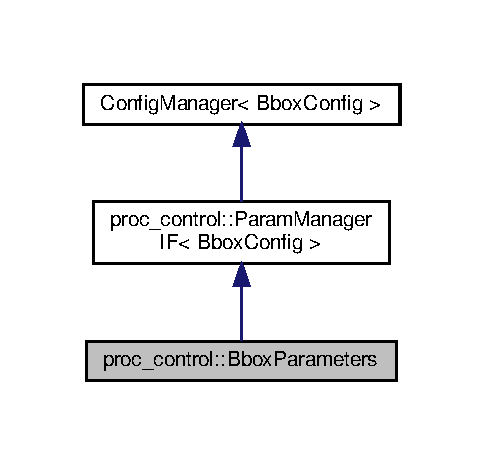
\includegraphics[width=232pt]{classproc__control_1_1_bbox_parameters__inherit__graph}
\end{center}
\end{figure}


Collaboration diagram for proc\+\_\+control\+:\+:Bbox\+Parameters\+:\nopagebreak
\begin{figure}[H]
\begin{center}
\leavevmode
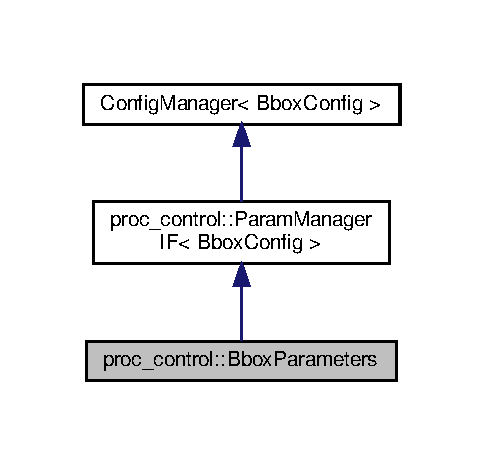
\includegraphics[width=232pt]{classproc__control_1_1_bbox_parameters__coll__graph}
\end{center}
\end{figure}
\subsection*{Public Member Functions}
\begin{DoxyCompactItemize}
\item 
\mbox{\Hypertarget{classproc__control_1_1_bbox_parameters_a50eb03ac9ebdf9fc7cfd5efc67d87856}\label{classproc__control_1_1_bbox_parameters_a50eb03ac9ebdf9fc7cfd5efc67d87856}} 
{\bfseries Bbox\+Parameters} (std\+::string axe\+\_\+name, std\+::shared\+\_\+ptr$<$ std\+::vector$<$ double $>$$>$ \&bbox\+Parameters)
\item 
\mbox{\Hypertarget{classproc__control_1_1_bbox_parameters_a114e932b6dfde1b4acfddc87c2a28038}\label{classproc__control_1_1_bbox_parameters_a114e932b6dfde1b4acfddc87c2a28038}} 
void {\bfseries On\+Dynamic\+Reconfigure\+Change} (const Bbox\+Config \&config) override
\item 
\mbox{\Hypertarget{classproc__control_1_1_bbox_parameters_a4528ed0506741ee73524c0efad5bc6d9}\label{classproc__control_1_1_bbox_parameters_a4528ed0506741ee73524c0efad5bc6d9}} 
void {\bfseries Write\+Config\+File} (const Bbox\+Config \&config) override
\item 
\mbox{\Hypertarget{classproc__control_1_1_bbox_parameters_a62e2f1398edeaf66ea54453a97a7f124}\label{classproc__control_1_1_bbox_parameters_a62e2f1398edeaf66ea54453a97a7f124}} 
void {\bfseries Read\+Config\+File} (Bbox\+Config \&config) override
\end{DoxyCompactItemize}
\subsection*{Additional Inherited Members}


The documentation for this class was generated from the following files\+:\begin{DoxyCompactItemize}
\item 
Parameters\+Manager/Bbox\+Parameters.\+h\item 
Parameters\+Manager/Bbox\+Parameters.\+cc\end{DoxyCompactItemize}

\hypertarget{classproc__control_1_1_b_controller}{}\section{proc\+\_\+control\+:\+:B\+Controller Class Reference}
\label{classproc__control_1_1_b_controller}\index{proc\+\_\+control\+::\+B\+Controller@{proc\+\_\+control\+::\+B\+Controller}}


Inheritance diagram for proc\+\_\+control\+:\+:B\+Controller\+:\nopagebreak
\begin{figure}[H]
\begin{center}
\leavevmode
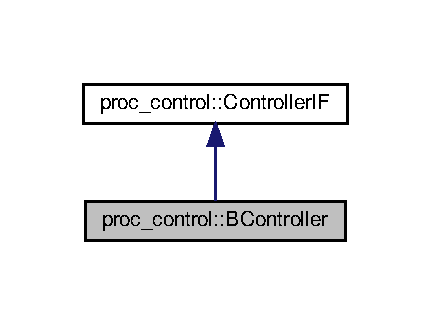
\includegraphics[width=207pt]{classproc__control_1_1_b_controller__inherit__graph}
\end{center}
\end{figure}


Collaboration diagram for proc\+\_\+control\+:\+:B\+Controller\+:\nopagebreak
\begin{figure}[H]
\begin{center}
\leavevmode
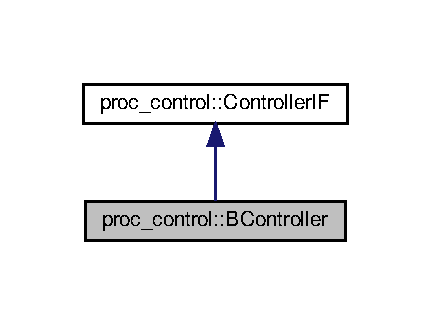
\includegraphics[width=207pt]{classproc__control_1_1_b_controller__coll__graph}
\end{center}
\end{figure}
\subsection*{Public Member Functions}
\begin{DoxyCompactItemize}
\item 
\mbox{\Hypertarget{classproc__control_1_1_b_controller_adb50beebef154358a61f25255cfcae0e}\label{classproc__control_1_1_b_controller_adb50beebef154358a61f25255cfcae0e}} 
Eigen\+::\+Vector\+Xd {\bfseries Computed\+Wrench\+From\+Error} (control\+::\+Controller\+C\+MD \&command) override
\end{DoxyCompactItemize}


The documentation for this class was generated from the following files\+:\begin{DoxyCompactItemize}
\item 
Controller/B\+Controller.\+h\item 
Controller/B\+Controller.\+cc\end{DoxyCompactItemize}

\hypertarget{classproc__control_1_1_command_b_parameters}{}\section{proc\+\_\+control\+:\+:Command\+B\+Parameters Class Reference}
\label{classproc__control_1_1_command_b_parameters}\index{proc\+\_\+control\+::\+Command\+B\+Parameters@{proc\+\_\+control\+::\+Command\+B\+Parameters}}
\subsection*{Public Member Functions}
\begin{DoxyCompactItemize}
\item 
\mbox{\Hypertarget{classproc__control_1_1_command_b_parameters_a584df157697192334ec328df86440b88}\label{classproc__control_1_1_command_b_parameters_a584df157697192334ec328df86440b88}} 
{\bfseries Command\+B\+Parameters} (std\+::shared\+\_\+ptr$<$ control\+::\+Transfer\+Function\+Coefficient $>$ \&transfer\+Function\+CoefficientB)
\end{DoxyCompactItemize}


The documentation for this class was generated from the following files\+:\begin{DoxyCompactItemize}
\item 
Parameters\+Manager/Command\+B\+Parameters.\+h\item 
Parameters\+Manager/Command\+B\+Parameters.\+cc\end{DoxyCompactItemize}

\hypertarget{class_config_manager}{}\section{Config\+Manager$<$ T $>$ Class Template Reference}
\label{class_config_manager}\index{Config\+Manager$<$ T $>$@{Config\+Manager$<$ T $>$}}


Inheritance diagram for Config\+Manager$<$ T $>$\+:\nopagebreak
\begin{figure}[H]
\begin{center}
\leavevmode
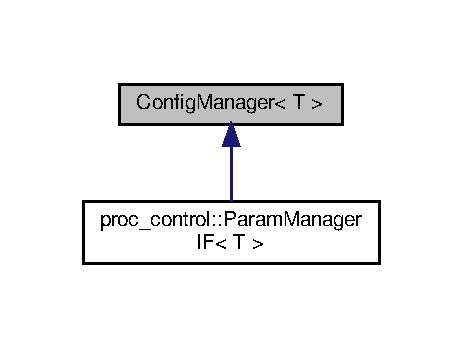
\includegraphics[width=222pt]{class_config_manager__inherit__graph}
\end{center}
\end{figure}
\subsection*{Protected Member Functions}
\begin{DoxyCompactItemize}
\item 
\mbox{\Hypertarget{class_config_manager_a1237cc0ba9d19c05c5d284b28742b87a}\label{class_config_manager_a1237cc0ba9d19c05c5d284b28742b87a}} 
{\bfseries Config\+Manager} (const std\+::string \&manager\+\_\+name)
\item 
\mbox{\Hypertarget{class_config_manager_a3fff642da4bd73a5d64bb90e8ae85915}\label{class_config_manager_a3fff642da4bd73a5d64bb90e8ae85915}} 
void {\bfseries Init} ()
\item 
\mbox{\Hypertarget{class_config_manager_a6256f5de4d8f6e6c7a9d62f97926601d}\label{class_config_manager_a6256f5de4d8f6e6c7a9d62f97926601d}} 
virtual void {\bfseries On\+Dynamic\+Reconfigure\+Change} (const T \&config)=0
\item 
\mbox{\Hypertarget{class_config_manager_a4dfc5e51faba689ec20bf9f8d994c135}\label{class_config_manager_a4dfc5e51faba689ec20bf9f8d994c135}} 
virtual void {\bfseries Write\+Config\+File} (const T \&config)=0
\item 
\mbox{\Hypertarget{class_config_manager_af7302a9dd1d428cd6a2a365ddedf35ee}\label{class_config_manager_af7302a9dd1d428cd6a2a365ddedf35ee}} 
virtual void {\bfseries Read\+Config\+File} (T \&config)=0
\item 
\mbox{\Hypertarget{class_config_manager_ace20b48c9921f9771e5203e164b58b1b}\label{class_config_manager_ace20b48c9921f9771e5203e164b58b1b}} 
std\+::string {\bfseries Get\+Manager\+Name} ()
\end{DoxyCompactItemize}


The documentation for this class was generated from the following file\+:\begin{DoxyCompactItemize}
\item 
Config/\hyperlink{_config_manager_8h}{Config\+Manager.\+h}\end{DoxyCompactItemize}

\hypertarget{classproc__control_1_1_control_input}{}\section{proc\+\_\+control\+:\+:Control\+Input Class Reference}
\label{classproc__control_1_1_control_input}\index{proc\+\_\+control\+::\+Control\+Input@{proc\+\_\+control\+::\+Control\+Input}}
\subsection*{Public Member Functions}
\begin{DoxyCompactItemize}
\item 
\mbox{\Hypertarget{classproc__control_1_1_control_input_a7599f6620c8d4b61ced67ca9de195dbb}\label{classproc__control_1_1_control_input_a7599f6620c8d4b61ced67ca9de195dbb}} 
{\bfseries Control\+Input} (const ros\+::\+Node\+Handle\+Ptr \&nh)
\item 
\mbox{\Hypertarget{classproc__control_1_1_control_input_ad5757d3710f158a88aad9a7b70d87483}\label{classproc__control_1_1_control_input_ad5757d3710f158a88aad9a7b70d87483}} 
void {\bfseries Odometry\+Callback} (const nav\+\_\+msgs\+::\+Odometry\+::\+Const\+Ptr \&odom\+In)
\item 
\mbox{\Hypertarget{classproc__control_1_1_control_input_a7661dc7221a11d9db6ec41d88a8597f3}\label{classproc__control_1_1_control_input_a7661dc7221a11d9db6ec41d88a8597f3}} 
Eigen\+::\+Vector3d {\bfseries Get\+Pose\+Position} () const
\item 
\mbox{\Hypertarget{classproc__control_1_1_control_input_a8dcaf4b6b888b3e4282b45c84f9830cd}\label{classproc__control_1_1_control_input_a8dcaf4b6b888b3e4282b45c84f9830cd}} 
Eigen\+::\+Vector3d {\bfseries Get\+Twist\+Linear} () const
\item 
\mbox{\Hypertarget{classproc__control_1_1_control_input_a48426014ee76df6f552244146cd90b4a}\label{classproc__control_1_1_control_input_a48426014ee76df6f552244146cd90b4a}} 
Eigen\+::\+Vector3d {\bfseries Get\+Pose\+Orientation} () const
\item 
\mbox{\Hypertarget{classproc__control_1_1_control_input_a6cd6d9cc0a2d472d3b393c05d7b30a50}\label{classproc__control_1_1_control_input_a6cd6d9cc0a2d472d3b393c05d7b30a50}} 
Eigen\+::\+Vector3d {\bfseries Get\+Twist\+Angular} () const
\end{DoxyCompactItemize}
\subsection*{Public Attributes}
\begin{DoxyCompactItemize}
\item 
\mbox{\Hypertarget{classproc__control_1_1_control_input_a9d7518257f6d068be167e3b0878dc032}\label{classproc__control_1_1_control_input_a9d7518257f6d068be167e3b0878dc032}} 
const double {\bfseries D\+E\+G\+R\+E\+E\+\_\+\+T\+O\+\_\+\+R\+AD} = M\+\_\+\+PI / 180.\+0
\end{DoxyCompactItemize}


The documentation for this class was generated from the following files\+:\begin{DoxyCompactItemize}
\item 
Control\+Input/\hyperlink{_control_input_8h}{Control\+Input.\+h}\item 
Control\+Input/\hyperlink{_control_input_8cc}{Control\+Input.\+cc}\end{DoxyCompactItemize}

\hypertarget{classproc__control_1_1_controller_i_f}{}\section{proc\+\_\+control\+:\+:Controller\+IF Class Reference}
\label{classproc__control_1_1_controller_i_f}\index{proc\+\_\+control\+::\+Controller\+IF@{proc\+\_\+control\+::\+Controller\+IF}}


Inheritance diagram for proc\+\_\+control\+:\+:Controller\+IF\+:\nopagebreak
\begin{figure}[H]
\begin{center}
\leavevmode
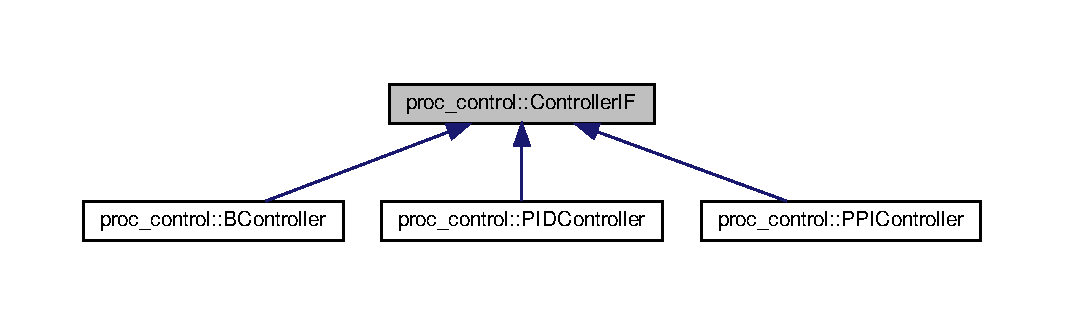
\includegraphics[width=350pt]{classproc__control_1_1_controller_i_f__inherit__graph}
\end{center}
\end{figure}
\subsection*{Public Member Functions}
\begin{DoxyCompactItemize}
\item 
\mbox{\Hypertarget{classproc__control_1_1_controller_i_f_a4abdd5192893128a0a07dd6cfed4c4cb}\label{classproc__control_1_1_controller_i_f_a4abdd5192893128a0a07dd6cfed4c4cb}} 
virtual Eigen\+::\+Vector\+Xd {\bfseries Computed\+Wrench\+From\+Error} (control\+::\+Controller\+C\+MD \&command)=0
\end{DoxyCompactItemize}


The documentation for this class was generated from the following file\+:\begin{DoxyCompactItemize}
\item 
Controller/Controller\+I\+F.\+h\end{DoxyCompactItemize}

\hypertarget{classproc__control_1_1_control_mode_i_f}{}\section{proc\+\_\+control\+:\+:Control\+Mode\+IF Class Reference}
\label{classproc__control_1_1_control_mode_i_f}\index{proc\+\_\+control\+::\+Control\+Mode\+IF@{proc\+\_\+control\+::\+Control\+Mode\+IF}}


Inheritance diagram for proc\+\_\+control\+:\+:Control\+Mode\+IF\+:\nopagebreak
\begin{figure}[H]
\begin{center}
\leavevmode
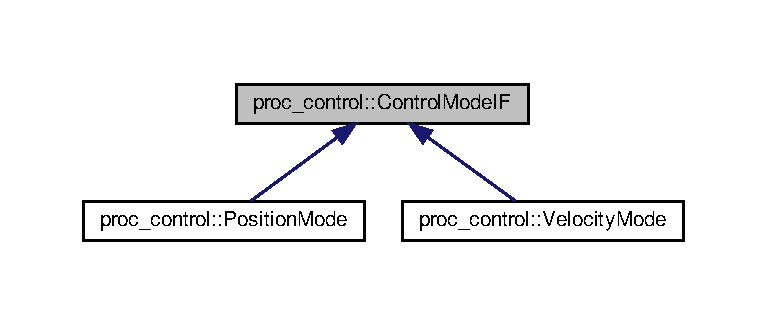
\includegraphics[width=350pt]{classproc__control_1_1_control_mode_i_f__inherit__graph}
\end{center}
\end{figure}
\subsection*{Public Member Functions}
\begin{DoxyCompactItemize}
\item 
\mbox{\Hypertarget{classproc__control_1_1_control_mode_i_f_a7a42e32ea4bb6857ffbd9218b8941e8f}\label{classproc__control_1_1_control_mode_i_f_a7a42e32ea4bb6857ffbd9218b8941e8f}} 
virtual void {\bfseries Process} ()=0
\item 
\mbox{\Hypertarget{classproc__control_1_1_control_mode_i_f_a262e9386519da6be5915e9bf876adfce}\label{classproc__control_1_1_control_mode_i_f_a262e9386519da6be5915e9bf876adfce}} 
virtual void {\bfseries Set\+Target} (bool is\+Global, Eigen\+::\+Vector\+Xd \&target\+Pose)=0
\item 
\mbox{\Hypertarget{classproc__control_1_1_control_mode_i_f_aef8533875572c59470de62e79b258672}\label{classproc__control_1_1_control_mode_i_f_aef8533875572c59470de62e79b258672}} 
virtual void {\bfseries Set\+Decoupled\+Target} (bool is\+Global, const std\+::vector$<$ bool $>$ \&keep\+Target, Eigen\+::\+Vector\+Xd \&target\+Pose)=0
\end{DoxyCompactItemize}


The documentation for this class was generated from the following file\+:\begin{DoxyCompactItemize}
\item 
Mode/\hyperlink{_control_mode_i_f_8h}{Control\+Mode\+I\+F.\+h}\end{DoxyCompactItemize}

\hypertarget{classproc__control_1_1_param_manager_i_f}{}\section{proc\+\_\+control\+:\+:Param\+Manager\+IF$<$ T $>$ Class Template Reference}
\label{classproc__control_1_1_param_manager_i_f}\index{proc\+\_\+control\+::\+Param\+Manager\+I\+F$<$ T $>$@{proc\+\_\+control\+::\+Param\+Manager\+I\+F$<$ T $>$}}


Inheritance diagram for proc\+\_\+control\+:\+:Param\+Manager\+IF$<$ T $>$\+:\nopagebreak
\begin{figure}[H]
\begin{center}
\leavevmode
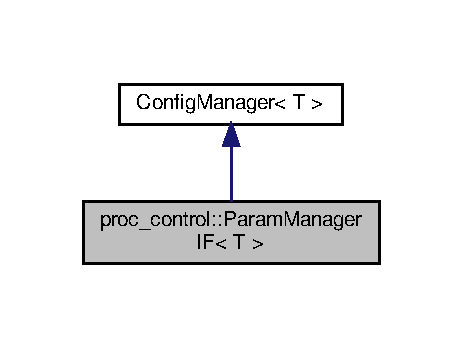
\includegraphics[width=222pt]{classproc__control_1_1_param_manager_i_f__inherit__graph}
\end{center}
\end{figure}


Collaboration diagram for proc\+\_\+control\+:\+:Param\+Manager\+IF$<$ T $>$\+:\nopagebreak
\begin{figure}[H]
\begin{center}
\leavevmode
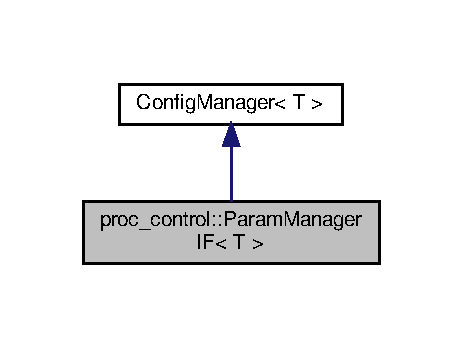
\includegraphics[width=222pt]{classproc__control_1_1_param_manager_i_f__coll__graph}
\end{center}
\end{figure}
\subsection*{Public Member Functions}
\begin{DoxyCompactItemize}
\item 
\mbox{\Hypertarget{classproc__control_1_1_param_manager_i_f_aaa30f9f70b14c3341b3ff597cdda4726}\label{classproc__control_1_1_param_manager_i_f_aaa30f9f70b14c3341b3ff597cdda4726}} 
{\bfseries Param\+Manager\+IF} (const std\+::string \&param\+Name)
\item 
\mbox{\Hypertarget{classproc__control_1_1_param_manager_i_f_a45bc4d1c2312f1a49daae4cdc6ca7d6d}\label{classproc__control_1_1_param_manager_i_f_a45bc4d1c2312f1a49daae4cdc6ca7d6d}} 
virtual void {\bfseries On\+Dynamic\+Reconfigure\+Change} (const T \&config)=0
\item 
\mbox{\Hypertarget{classproc__control_1_1_param_manager_i_f_a84dd599146e16a8595b1e7a3d22b05d9}\label{classproc__control_1_1_param_manager_i_f_a84dd599146e16a8595b1e7a3d22b05d9}} 
virtual void {\bfseries Write\+Config\+File} (const T \&config)=0
\item 
\mbox{\Hypertarget{classproc__control_1_1_param_manager_i_f_a79139c3be12afdff3ab3fa46eea00bbd}\label{classproc__control_1_1_param_manager_i_f_a79139c3be12afdff3ab3fa46eea00bbd}} 
virtual void {\bfseries Read\+Config\+File} (T \&config)=0
\end{DoxyCompactItemize}
\subsection*{Additional Inherited Members}


The documentation for this class was generated from the following file\+:\begin{DoxyCompactItemize}
\item 
Parameters\+Manager/Param\+Manager\+I\+F.\+h\end{DoxyCompactItemize}

\hypertarget{classproc__control_1_1_p_i_d_controller}{}\section{proc\+\_\+control\+:\+:P\+I\+D\+Controller Class Reference}
\label{classproc__control_1_1_p_i_d_controller}\index{proc\+\_\+control\+::\+P\+I\+D\+Controller@{proc\+\_\+control\+::\+P\+I\+D\+Controller}}


Inheritance diagram for proc\+\_\+control\+:\+:P\+I\+D\+Controller\+:\nopagebreak
\begin{figure}[H]
\begin{center}
\leavevmode
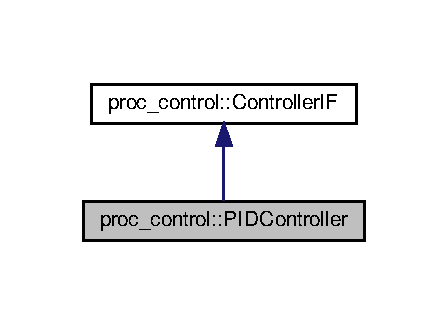
\includegraphics[width=215pt]{classproc__control_1_1_p_i_d_controller__inherit__graph}
\end{center}
\end{figure}


Collaboration diagram for proc\+\_\+control\+:\+:P\+I\+D\+Controller\+:\nopagebreak
\begin{figure}[H]
\begin{center}
\leavevmode
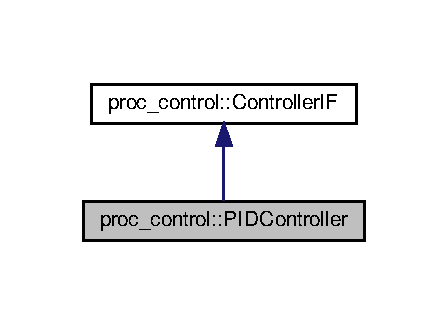
\includegraphics[width=215pt]{classproc__control_1_1_p_i_d_controller__coll__graph}
\end{center}
\end{figure}
\subsection*{Public Member Functions}
\begin{DoxyCompactItemize}
\item 
\mbox{\Hypertarget{classproc__control_1_1_p_i_d_controller_a4f76acfe174b826405f4509179b0dbe5}\label{classproc__control_1_1_p_i_d_controller_a4f76acfe174b826405f4509179b0dbe5}} 
{\bfseries P\+I\+D\+Controller} (const std\+::string \&controller\+Type)
\item 
\mbox{\Hypertarget{classproc__control_1_1_p_i_d_controller_af7cee6701ec98ebbead8429ce466cfaa}\label{classproc__control_1_1_p_i_d_controller_af7cee6701ec98ebbead8429ce466cfaa}} 
Eigen\+::\+Vector\+Xd {\bfseries Computed\+Wrench\+From\+Error} (control\+::\+Controller\+C\+MD \&command) override
\end{DoxyCompactItemize}


The documentation for this class was generated from the following files\+:\begin{DoxyCompactItemize}
\item 
Controller/P\+I\+D\+Controller.\+h\item 
Controller/P\+I\+D\+Controller.\+cc\end{DoxyCompactItemize}

\hypertarget{classproc__control_1_1_p_i_d_parameters}{}\section{proc\+\_\+control\+:\+:P\+I\+D\+Parameters Class Reference}
\label{classproc__control_1_1_p_i_d_parameters}\index{proc\+\_\+control\+::\+P\+I\+D\+Parameters@{proc\+\_\+control\+::\+P\+I\+D\+Parameters}}


Inheritance diagram for proc\+\_\+control\+:\+:P\+I\+D\+Parameters\+:\nopagebreak
\begin{figure}[H]
\begin{center}
\leavevmode
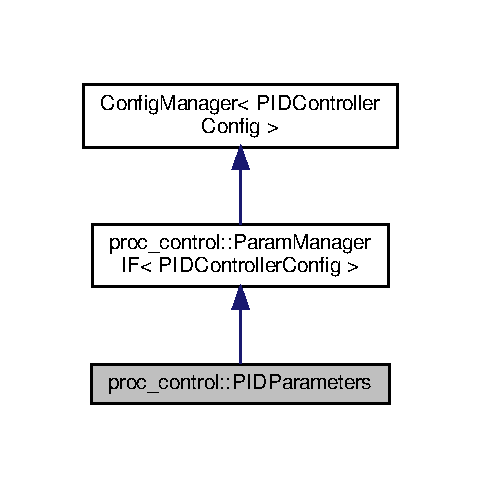
\includegraphics[width=231pt]{classproc__control_1_1_p_i_d_parameters__inherit__graph}
\end{center}
\end{figure}


Collaboration diagram for proc\+\_\+control\+:\+:P\+I\+D\+Parameters\+:\nopagebreak
\begin{figure}[H]
\begin{center}
\leavevmode
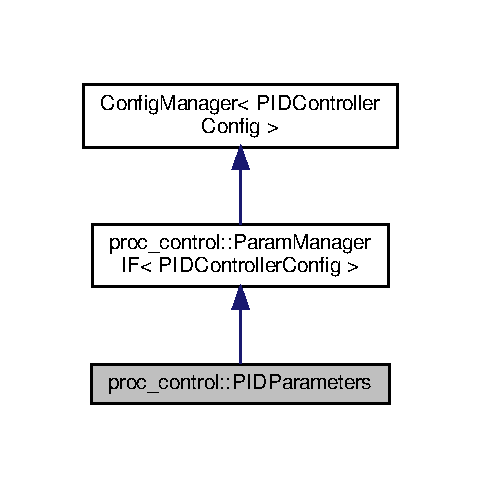
\includegraphics[width=231pt]{classproc__control_1_1_p_i_d_parameters__coll__graph}
\end{center}
\end{figure}
\subsection*{Public Member Functions}
\begin{DoxyCompactItemize}
\item 
\mbox{\Hypertarget{classproc__control_1_1_p_i_d_parameters_a3441450a67dbc26fbb2c2db1b47c035e}\label{classproc__control_1_1_p_i_d_parameters_a3441450a67dbc26fbb2c2db1b47c035e}} 
{\bfseries P\+I\+D\+Parameters} (std\+::string axe\+\_\+name, std\+::string mode, std\+::shared\+\_\+ptr$<$ control\+::\+P\+I\+D\+Parameters $>$ \&pid\+Parameters)
\item 
\mbox{\Hypertarget{classproc__control_1_1_p_i_d_parameters_a5e1bf35f716a3b7c734b7e596dd72810}\label{classproc__control_1_1_p_i_d_parameters_a5e1bf35f716a3b7c734b7e596dd72810}} 
void {\bfseries On\+Dynamic\+Reconfigure\+Change} (const P\+I\+D\+Controller\+Config \&config) override
\item 
\mbox{\Hypertarget{classproc__control_1_1_p_i_d_parameters_a3dbcf89841eec59edd9b9e47fcc71273}\label{classproc__control_1_1_p_i_d_parameters_a3dbcf89841eec59edd9b9e47fcc71273}} 
void {\bfseries Write\+Config\+File} (const P\+I\+D\+Controller\+Config \&config) override
\item 
\mbox{\Hypertarget{classproc__control_1_1_p_i_d_parameters_aeaebb55d9aebec7a576121258241fe0e}\label{classproc__control_1_1_p_i_d_parameters_aeaebb55d9aebec7a576121258241fe0e}} 
void {\bfseries Read\+Config\+File} (P\+I\+D\+Controller\+Config \&config) override
\item 
\mbox{\Hypertarget{classproc__control_1_1_p_i_d_parameters_aea85a45d3a5a1b8ef7f65b4e354dbf07}\label{classproc__control_1_1_p_i_d_parameters_aea85a45d3a5a1b8ef7f65b4e354dbf07}} 
double {\bfseries Get\+Constante\+Depth\+Force} ()
\item 
\mbox{\Hypertarget{classproc__control_1_1_p_i_d_parameters_a894c72328645382879c55a83d597db5d}\label{classproc__control_1_1_p_i_d_parameters_a894c72328645382879c55a83d597db5d}} 
std\+::shared\+\_\+ptr$<$ control\+::\+P\+I\+D\+Parameters $>$ \& {\bfseries Get\+P\+I\+D\+Parameters} ()
\end{DoxyCompactItemize}
\subsection*{Additional Inherited Members}


The documentation for this class was generated from the following files\+:\begin{DoxyCompactItemize}
\item 
Parameters\+Manager/P\+I\+D\+Parameters.\+h\item 
Parameters\+Manager/P\+I\+D\+Parameters.\+cc\end{DoxyCompactItemize}

\hypertarget{classproc__control_1_1_position_mode}{}\section{proc\+\_\+control\+:\+:Position\+Mode Class Reference}
\label{classproc__control_1_1_position_mode}\index{proc\+\_\+control\+::\+Position\+Mode@{proc\+\_\+control\+::\+Position\+Mode}}


Inheritance diagram for proc\+\_\+control\+:\+:Position\+Mode\+:\nopagebreak
\begin{figure}[H]
\begin{center}
\leavevmode
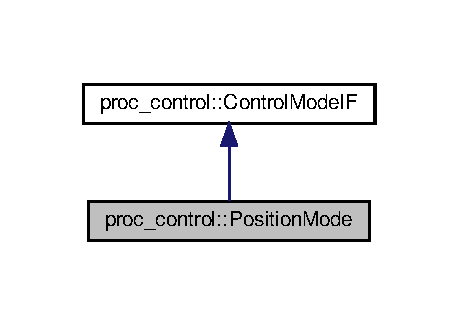
\includegraphics[width=220pt]{classproc__control_1_1_position_mode__inherit__graph}
\end{center}
\end{figure}


Collaboration diagram for proc\+\_\+control\+:\+:Position\+Mode\+:\nopagebreak
\begin{figure}[H]
\begin{center}
\leavevmode
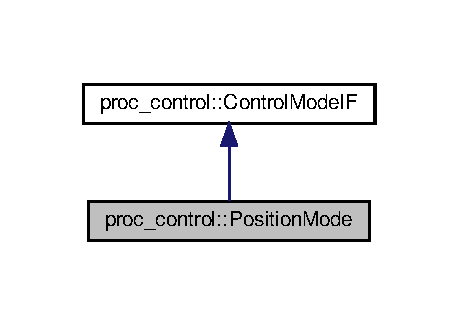
\includegraphics[width=220pt]{classproc__control_1_1_position_mode__coll__graph}
\end{center}
\end{figure}
\subsection*{Public Member Functions}
\begin{DoxyCompactItemize}
\item 
\mbox{\Hypertarget{classproc__control_1_1_position_mode_aa0f0beda66599f422d0d2ea44fe9d1e1}\label{classproc__control_1_1_position_mode_aa0f0beda66599f422d0d2ea44fe9d1e1}} 
{\bfseries Position\+Mode} (std\+::shared\+\_\+ptr$<$ \hyperlink{classproc__control_1_1_robot_state}{Robot\+State} $>$ \&robot\+State, std\+::unique\+\_\+ptr$<$ \hyperlink{classproc__control_1_1_controller_i_f}{Controller\+IF} $>$ \&control\+A\+UV)
\item 
\mbox{\Hypertarget{classproc__control_1_1_position_mode_a02d5e57b88eb2fc00e8b1eb2111a1f4f}\label{classproc__control_1_1_position_mode_a02d5e57b88eb2fc00e8b1eb2111a1f4f}} 
void {\bfseries Process} () override
\item 
\mbox{\Hypertarget{classproc__control_1_1_position_mode_a35aedca126be447584bf44be01d66cd5}\label{classproc__control_1_1_position_mode_a35aedca126be447584bf44be01d66cd5}} 
void {\bfseries Set\+Target} (bool is\+Global, Eigen\+::\+Vector\+Xd \&target\+Pose) override
\item 
\mbox{\Hypertarget{classproc__control_1_1_position_mode_a7f2224eb7984c83509ff961b97e71078}\label{classproc__control_1_1_position_mode_a7f2224eb7984c83509ff961b97e71078}} 
void {\bfseries Set\+Decoupled\+Target} (bool is\+Global, const std\+::vector$<$ bool $>$ \&keep\+Target, Eigen\+::\+Vector\+Xd \&target\+Pose) override
\end{DoxyCompactItemize}


The documentation for this class was generated from the following files\+:\begin{DoxyCompactItemize}
\item 
Mode/\hyperlink{_position_mode_8h}{Position\+Mode.\+h}\item 
Mode/\hyperlink{_position_mode_8cc}{Position\+Mode.\+cc}\end{DoxyCompactItemize}

\hypertarget{classproc__control_1_1_p_p_i_controller}{}\section{proc\+\_\+control\+:\+:P\+P\+I\+Controller Class Reference}
\label{classproc__control_1_1_p_p_i_controller}\index{proc\+\_\+control\+::\+P\+P\+I\+Controller@{proc\+\_\+control\+::\+P\+P\+I\+Controller}}


Inheritance diagram for proc\+\_\+control\+:\+:P\+P\+I\+Controller\+:\nopagebreak
\begin{figure}[H]
\begin{center}
\leavevmode
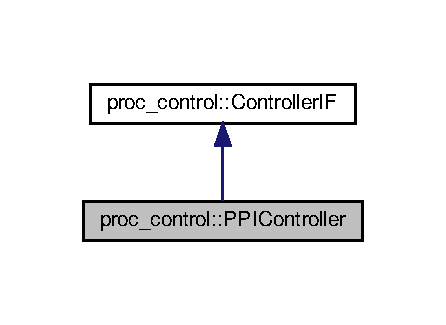
\includegraphics[width=214pt]{classproc__control_1_1_p_p_i_controller__inherit__graph}
\end{center}
\end{figure}


Collaboration diagram for proc\+\_\+control\+:\+:P\+P\+I\+Controller\+:\nopagebreak
\begin{figure}[H]
\begin{center}
\leavevmode
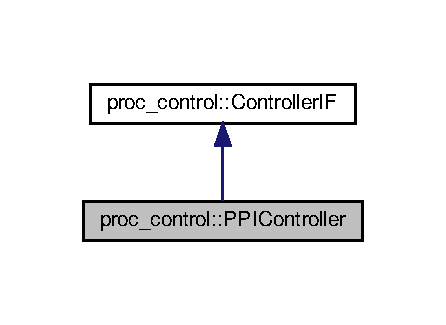
\includegraphics[width=214pt]{classproc__control_1_1_p_p_i_controller__coll__graph}
\end{center}
\end{figure}
\subsection*{Public Member Functions}
\begin{DoxyCompactItemize}
\item 
\mbox{\Hypertarget{classproc__control_1_1_p_p_i_controller_a9299c3beded1afa65de537e08b5ad841}\label{classproc__control_1_1_p_p_i_controller_a9299c3beded1afa65de537e08b5ad841}} 
Eigen\+::\+Vector\+Xd {\bfseries Computed\+Wrench\+From\+Error} (control\+::\+Controller\+C\+MD \&command) override
\end{DoxyCompactItemize}


The documentation for this class was generated from the following files\+:\begin{DoxyCompactItemize}
\item 
Controller/P\+P\+I\+Controller.\+h\item 
Controller/P\+P\+I\+Controller.\+cc\end{DoxyCompactItemize}

\hypertarget{classproc__control_1_1_p_p_i_parameters}{}\section{proc\+\_\+control\+:\+:P\+P\+I\+Parameters Class Reference}
\label{classproc__control_1_1_p_p_i_parameters}\index{proc\+\_\+control\+::\+P\+P\+I\+Parameters@{proc\+\_\+control\+::\+P\+P\+I\+Parameters}}


Inheritance diagram for proc\+\_\+control\+:\+:P\+P\+I\+Parameters\+:\nopagebreak
\begin{figure}[H]
\begin{center}
\leavevmode
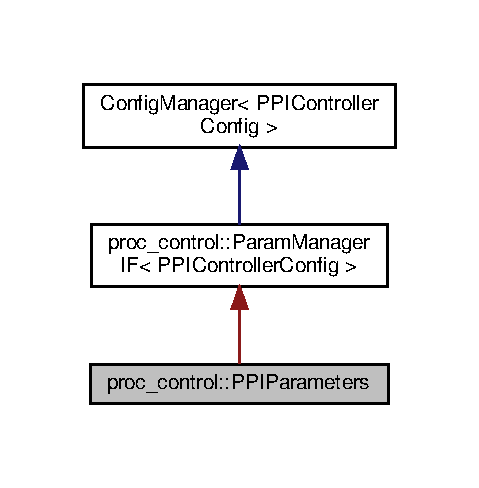
\includegraphics[width=230pt]{classproc__control_1_1_p_p_i_parameters__inherit__graph}
\end{center}
\end{figure}


Collaboration diagram for proc\+\_\+control\+:\+:P\+P\+I\+Parameters\+:\nopagebreak
\begin{figure}[H]
\begin{center}
\leavevmode
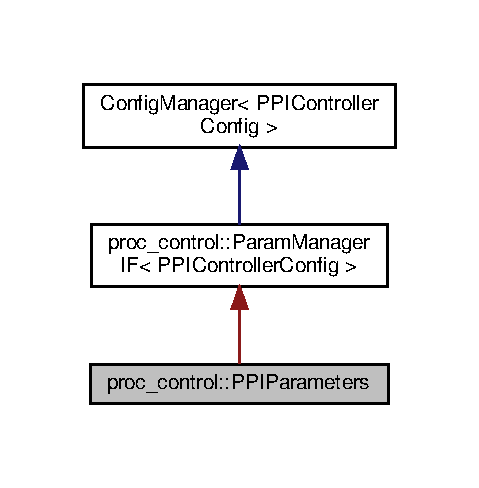
\includegraphics[width=230pt]{classproc__control_1_1_p_p_i_parameters__coll__graph}
\end{center}
\end{figure}
\subsection*{Public Member Functions}
\begin{DoxyCompactItemize}
\item 
\mbox{\Hypertarget{classproc__control_1_1_p_p_i_parameters_a87b8ca194a8b226c7a5ffac255394c86}\label{classproc__control_1_1_p_p_i_parameters_a87b8ca194a8b226c7a5ffac255394c86}} 
{\bfseries P\+P\+I\+Parameters} (const std\+::string \&param\+Name, std\+::shared\+\_\+ptr$<$ control\+::\+Transfer\+Function\+Coefficient $>$ \&transfer\+Function\+Coefficient)
\item 
\mbox{\Hypertarget{classproc__control_1_1_p_p_i_parameters_aa9373a82f26917cedef0c36f9246174b}\label{classproc__control_1_1_p_p_i_parameters_aa9373a82f26917cedef0c36f9246174b}} 
void {\bfseries On\+Dynamic\+Reconfigure\+Change} (const P\+P\+I\+Controller\+Config \&config) override
\item 
\mbox{\Hypertarget{classproc__control_1_1_p_p_i_parameters_a03b3e06540ea1e11796be7e1461842d9}\label{classproc__control_1_1_p_p_i_parameters_a03b3e06540ea1e11796be7e1461842d9}} 
void {\bfseries Write\+Config\+File} (const P\+P\+I\+Controller\+Config \&config) override
\item 
\mbox{\Hypertarget{classproc__control_1_1_p_p_i_parameters_aa6e22022871b0a7e6a972a20f757d6e3}\label{classproc__control_1_1_p_p_i_parameters_aa6e22022871b0a7e6a972a20f757d6e3}} 
void {\bfseries Read\+Config\+File} (P\+P\+I\+Controller\+Config \&config) override
\end{DoxyCompactItemize}


The documentation for this class was generated from the following files\+:\begin{DoxyCompactItemize}
\item 
Parameters\+Manager/P\+P\+I\+Parameters.\+h\item 
Parameters\+Manager/P\+P\+I\+Parameters.\+cc\end{DoxyCompactItemize}

\hypertarget{classproc__control_1_1_proc_control_node}{}\section{proc\+\_\+control\+:\+:Proc\+Control\+Node Class Reference}
\label{classproc__control_1_1_proc_control_node}\index{proc\+\_\+control\+::\+Proc\+Control\+Node@{proc\+\_\+control\+::\+Proc\+Control\+Node}}
\subsection*{Public Member Functions}
\begin{DoxyCompactItemize}
\item 
\hyperlink{classproc__control_1_1_proc_control_node_a3990253ca2e924c15e25cecba4297359}{Proc\+Control\+Node} (const ros\+::\+Node\+Handle\+Ptr \&nh)
\item 
\hyperlink{classproc__control_1_1_proc_control_node_ac4ec58d30c4c8a5842f1797154b6e363}{$\sim$\+Proc\+Control\+Node} ()
\item 
void \hyperlink{classproc__control_1_1_proc_control_node_adc8a2178d41c620f69cb74c2f09097cd}{Control\+Loop} ()
\item 
bool \hyperlink{classproc__control_1_1_proc_control_node_ac56aa1e6e028c225be157371aba76d32}{Set\+Control\+Mode\+Callback} (proc\+\_\+control\+::\+Set\+Control\+Mode\+Request \&request, proc\+\_\+control\+::\+Set\+Control\+Mode\+Response \&response)
\item 
bool \hyperlink{classproc__control_1_1_proc_control_node_a7890db7144358d5aaf0daa7bfefed964}{Set\+Global\+Target\+Position\+Callback} (proc\+\_\+control\+::\+Set\+Position\+Target\+Request \&request, proc\+\_\+control\+::\+Set\+Position\+Target\+Response \&response)
\item 
bool \hyperlink{classproc__control_1_1_proc_control_node_ad331887883a3c1c44472d72dfced3db6}{Set\+Local\+Target\+Position\+Callback} (proc\+\_\+control\+::\+Set\+Position\+Target\+Request \&request, proc\+\_\+control\+::\+Set\+Position\+Target\+Response \&response)
\item 
bool \hyperlink{classproc__control_1_1_proc_control_node_a841b03177a02e542bf7f7aa8403c5382}{Set\+Global\+Decoupled\+Target\+Position\+Callback} (proc\+\_\+control\+::\+Set\+Decoupled\+Target\+Request \&request, proc\+\_\+control\+::\+Set\+Decoupled\+Target\+Response \&response)
\item 
bool \hyperlink{classproc__control_1_1_proc_control_node_a01301ec4fcd9e4d149994cbe27ff8ca1}{Set\+Local\+Decoupled\+Target\+Position\+Callback} (proc\+\_\+control\+::\+Set\+Decoupled\+Target\+Request \&request, proc\+\_\+control\+::\+Set\+Decoupled\+Target\+Response \&response)
\end{DoxyCompactItemize}
\subsection*{Public Attributes}
\begin{DoxyCompactItemize}
\item 
\mbox{\Hypertarget{classproc__control_1_1_proc_control_node_a5e3562edaa6eba1d9bf3cc9b17afbd8a}\label{classproc__control_1_1_proc_control_node_a5e3562edaa6eba1d9bf3cc9b17afbd8a}} 
const bool {\bfseries Global\+Target} = true
\item 
\mbox{\Hypertarget{classproc__control_1_1_proc_control_node_a9de14df77c66166cfaaaefa31726ea00}\label{classproc__control_1_1_proc_control_node_a9de14df77c66166cfaaaefa31726ea00}} 
const bool {\bfseries Local\+Target} = false
\end{DoxyCompactItemize}


\subsection{Constructor \& Destructor Documentation}
\mbox{\Hypertarget{classproc__control_1_1_proc_control_node_a3990253ca2e924c15e25cecba4297359}\label{classproc__control_1_1_proc_control_node_a3990253ca2e924c15e25cecba4297359}} 
\index{proc\+\_\+control\+::\+Proc\+Control\+Node@{proc\+\_\+control\+::\+Proc\+Control\+Node}!Proc\+Control\+Node@{Proc\+Control\+Node}}
\index{Proc\+Control\+Node@{Proc\+Control\+Node}!proc\+\_\+control\+::\+Proc\+Control\+Node@{proc\+\_\+control\+::\+Proc\+Control\+Node}}
\subsubsection{\texorpdfstring{Proc\+Control\+Node()}{ProcControlNode()}}
{\footnotesize\ttfamily proc\+\_\+control\+::\+Proc\+Control\+Node\+::\+Proc\+Control\+Node (\begin{DoxyParamCaption}\item[{const ros\+::\+Node\+Handle\+Ptr \&}]{nh }\end{DoxyParamCaption})}

Constructor of the \hyperlink{classproc__control_1_1_proc_control_node}{Proc\+Control\+Node} object. 
\begin{DoxyParams}{Parameters}
{\em nh} & Node handler pointer. \\
\hline
\end{DoxyParams}
\mbox{\Hypertarget{classproc__control_1_1_proc_control_node_ac4ec58d30c4c8a5842f1797154b6e363}\label{classproc__control_1_1_proc_control_node_ac4ec58d30c4c8a5842f1797154b6e363}} 
\index{proc\+\_\+control\+::\+Proc\+Control\+Node@{proc\+\_\+control\+::\+Proc\+Control\+Node}!````~Proc\+Control\+Node@{$\sim$\+Proc\+Control\+Node}}
\index{````~Proc\+Control\+Node@{$\sim$\+Proc\+Control\+Node}!proc\+\_\+control\+::\+Proc\+Control\+Node@{proc\+\_\+control\+::\+Proc\+Control\+Node}}
\subsubsection{\texorpdfstring{$\sim$\+Proc\+Control\+Node()}{~ProcControlNode()}}
{\footnotesize\ttfamily proc\+\_\+control\+::\+Proc\+Control\+Node\+::$\sim$\+Proc\+Control\+Node (\begin{DoxyParamCaption}{ }\end{DoxyParamCaption})}

Destructor of the \hyperlink{classproc__control_1_1_proc_control_node}{Proc\+Control\+Node} object. Shutdown all the connections to the services needed. 

\subsection{Member Function Documentation}
\mbox{\Hypertarget{classproc__control_1_1_proc_control_node_adc8a2178d41c620f69cb74c2f09097cd}\label{classproc__control_1_1_proc_control_node_adc8a2178d41c620f69cb74c2f09097cd}} 
\index{proc\+\_\+control\+::\+Proc\+Control\+Node@{proc\+\_\+control\+::\+Proc\+Control\+Node}!Control\+Loop@{Control\+Loop}}
\index{Control\+Loop@{Control\+Loop}!proc\+\_\+control\+::\+Proc\+Control\+Node@{proc\+\_\+control\+::\+Proc\+Control\+Node}}
\subsubsection{\texorpdfstring{Control\+Loop()}{ControlLoop()}}
{\footnotesize\ttfamily void proc\+\_\+control\+::\+Proc\+Control\+Node\+::\+Control\+Loop (\begin{DoxyParamCaption}{ }\end{DoxyParamCaption})}

A simple function that set \hyperlink{classproc__control_1_1_robot_state}{Robot\+State} from input and process position mode. \mbox{\Hypertarget{classproc__control_1_1_proc_control_node_ac56aa1e6e028c225be157371aba76d32}\label{classproc__control_1_1_proc_control_node_ac56aa1e6e028c225be157371aba76d32}} 
\index{proc\+\_\+control\+::\+Proc\+Control\+Node@{proc\+\_\+control\+::\+Proc\+Control\+Node}!Set\+Control\+Mode\+Callback@{Set\+Control\+Mode\+Callback}}
\index{Set\+Control\+Mode\+Callback@{Set\+Control\+Mode\+Callback}!proc\+\_\+control\+::\+Proc\+Control\+Node@{proc\+\_\+control\+::\+Proc\+Control\+Node}}
\subsubsection{\texorpdfstring{Set\+Control\+Mode\+Callback()}{SetControlModeCallback()}}
{\footnotesize\ttfamily bool proc\+\_\+control\+::\+Proc\+Control\+Node\+::\+Set\+Control\+Mode\+Callback (\begin{DoxyParamCaption}\item[{proc\+\_\+control\+::\+Set\+Control\+Mode\+Request \&}]{request,  }\item[{proc\+\_\+control\+::\+Set\+Control\+Mode\+Response \&}]{response }\end{DoxyParamCaption})}

Callback used to change the control mode \+: position or P\+PI or speed. 
\begin{DoxyParams}{Parameters}
{\em request} & The new control mode requested (request.\+mode). \\
\hline
{\em response} & This parameter isn\textquotesingle{}t use. \\
\hline
\end{DoxyParams}
\begin{DoxyReturn}{Returns}
true 
\end{DoxyReturn}
\mbox{\Hypertarget{classproc__control_1_1_proc_control_node_a841b03177a02e542bf7f7aa8403c5382}\label{classproc__control_1_1_proc_control_node_a841b03177a02e542bf7f7aa8403c5382}} 
\index{proc\+\_\+control\+::\+Proc\+Control\+Node@{proc\+\_\+control\+::\+Proc\+Control\+Node}!Set\+Global\+Decoupled\+Target\+Position\+Callback@{Set\+Global\+Decoupled\+Target\+Position\+Callback}}
\index{Set\+Global\+Decoupled\+Target\+Position\+Callback@{Set\+Global\+Decoupled\+Target\+Position\+Callback}!proc\+\_\+control\+::\+Proc\+Control\+Node@{proc\+\_\+control\+::\+Proc\+Control\+Node}}
\subsubsection{\texorpdfstring{Set\+Global\+Decoupled\+Target\+Position\+Callback()}{SetGlobalDecoupledTargetPositionCallback()}}
{\footnotesize\ttfamily bool proc\+\_\+control\+::\+Proc\+Control\+Node\+::\+Set\+Global\+Decoupled\+Target\+Position\+Callback (\begin{DoxyParamCaption}\item[{proc\+\_\+control\+::\+Set\+Decoupled\+Target\+Request \&}]{request,  }\item[{proc\+\_\+control\+::\+Set\+Decoupled\+Target\+Response \&}]{response }\end{DoxyParamCaption})}

Callback used to set global decoupled target position. 
\begin{DoxyParams}{Parameters}
{\em request} & The new global decoupled target position requested (request.\+X, request.\+Y, request.\+Z, request.\+Y\+AW, request.\+R\+O\+LL, request.\+P\+I\+T\+CH, request.\+keepX, request.\+keepY, request.\+keepZ, request.\+keep\+R\+O\+LL, request.\+keep\+P\+I\+T\+CH, request.\+keep\+Y\+AW) \\
\hline
{\em response} & This parameter isn\textquotesingle{}t use. \\
\hline
\end{DoxyParams}
\begin{DoxyReturn}{Returns}
true 
\end{DoxyReturn}
\mbox{\Hypertarget{classproc__control_1_1_proc_control_node_a7890db7144358d5aaf0daa7bfefed964}\label{classproc__control_1_1_proc_control_node_a7890db7144358d5aaf0daa7bfefed964}} 
\index{proc\+\_\+control\+::\+Proc\+Control\+Node@{proc\+\_\+control\+::\+Proc\+Control\+Node}!Set\+Global\+Target\+Position\+Callback@{Set\+Global\+Target\+Position\+Callback}}
\index{Set\+Global\+Target\+Position\+Callback@{Set\+Global\+Target\+Position\+Callback}!proc\+\_\+control\+::\+Proc\+Control\+Node@{proc\+\_\+control\+::\+Proc\+Control\+Node}}
\subsubsection{\texorpdfstring{Set\+Global\+Target\+Position\+Callback()}{SetGlobalTargetPositionCallback()}}
{\footnotesize\ttfamily bool proc\+\_\+control\+::\+Proc\+Control\+Node\+::\+Set\+Global\+Target\+Position\+Callback (\begin{DoxyParamCaption}\item[{proc\+\_\+control\+::\+Set\+Position\+Target\+Request \&}]{request,  }\item[{proc\+\_\+control\+::\+Set\+Position\+Target\+Response \&}]{response }\end{DoxyParamCaption})}

Callback used to set global target position. 
\begin{DoxyParams}{Parameters}
{\em request} & The new global target position requested (request.\+X, request.\+Y, request.\+Z, request.\+Y\+AW, request.\+R\+O\+LL, request.\+P\+I\+T\+CH). \\
\hline
{\em response} & This parameter isn\textquotesingle{}t use. \\
\hline
\end{DoxyParams}
\begin{DoxyReturn}{Returns}
true 
\end{DoxyReturn}
\mbox{\Hypertarget{classproc__control_1_1_proc_control_node_a01301ec4fcd9e4d149994cbe27ff8ca1}\label{classproc__control_1_1_proc_control_node_a01301ec4fcd9e4d149994cbe27ff8ca1}} 
\index{proc\+\_\+control\+::\+Proc\+Control\+Node@{proc\+\_\+control\+::\+Proc\+Control\+Node}!Set\+Local\+Decoupled\+Target\+Position\+Callback@{Set\+Local\+Decoupled\+Target\+Position\+Callback}}
\index{Set\+Local\+Decoupled\+Target\+Position\+Callback@{Set\+Local\+Decoupled\+Target\+Position\+Callback}!proc\+\_\+control\+::\+Proc\+Control\+Node@{proc\+\_\+control\+::\+Proc\+Control\+Node}}
\subsubsection{\texorpdfstring{Set\+Local\+Decoupled\+Target\+Position\+Callback()}{SetLocalDecoupledTargetPositionCallback()}}
{\footnotesize\ttfamily bool proc\+\_\+control\+::\+Proc\+Control\+Node\+::\+Set\+Local\+Decoupled\+Target\+Position\+Callback (\begin{DoxyParamCaption}\item[{proc\+\_\+control\+::\+Set\+Decoupled\+Target\+Request \&}]{request,  }\item[{proc\+\_\+control\+::\+Set\+Decoupled\+Target\+Response \&}]{response }\end{DoxyParamCaption})}

Callback used to set local decoupled target position. 
\begin{DoxyParams}{Parameters}
{\em request} & The new global decoupled target position requested (request.\+X, request.\+Y, request.\+Z, request.\+Y\+AW, request.\+R\+O\+LL, request.\+P\+I\+T\+CH, request.\+keepX, request.\+keepY, request.\+keepZ, request.\+keep\+R\+O\+LL, request.\+keep\+P\+I\+T\+CH, request.\+keep\+Y\+AW) \\
\hline
{\em response} & This parameter isn\textquotesingle{}t use. \\
\hline
\end{DoxyParams}
\begin{DoxyReturn}{Returns}
true 
\end{DoxyReturn}
\mbox{\Hypertarget{classproc__control_1_1_proc_control_node_ad331887883a3c1c44472d72dfced3db6}\label{classproc__control_1_1_proc_control_node_ad331887883a3c1c44472d72dfced3db6}} 
\index{proc\+\_\+control\+::\+Proc\+Control\+Node@{proc\+\_\+control\+::\+Proc\+Control\+Node}!Set\+Local\+Target\+Position\+Callback@{Set\+Local\+Target\+Position\+Callback}}
\index{Set\+Local\+Target\+Position\+Callback@{Set\+Local\+Target\+Position\+Callback}!proc\+\_\+control\+::\+Proc\+Control\+Node@{proc\+\_\+control\+::\+Proc\+Control\+Node}}
\subsubsection{\texorpdfstring{Set\+Local\+Target\+Position\+Callback()}{SetLocalTargetPositionCallback()}}
{\footnotesize\ttfamily bool proc\+\_\+control\+::\+Proc\+Control\+Node\+::\+Set\+Local\+Target\+Position\+Callback (\begin{DoxyParamCaption}\item[{proc\+\_\+control\+::\+Set\+Position\+Target\+Request \&}]{request,  }\item[{proc\+\_\+control\+::\+Set\+Position\+Target\+Response \&}]{response }\end{DoxyParamCaption})}

Callback used to set local target position. 
\begin{DoxyParams}{Parameters}
{\em request} & The new local target position requested (request.\+X, request.\+Y, request.\+Z, request.\+Y\+AW, request.\+R\+O\+LL, request.\+P\+I\+T\+CH). \\
\hline
{\em response} & This parameter isn\textquotesingle{}t use. \\
\hline
\end{DoxyParams}
\begin{DoxyReturn}{Returns}
true 
\end{DoxyReturn}


The documentation for this class was generated from the following files\+:\begin{DoxyCompactItemize}
\item 
\hyperlink{proc__control__node_8h}{proc\+\_\+control\+\_\+node.\+h}\item 
\hyperlink{proc__control__node_8cc}{proc\+\_\+control\+\_\+node.\+cc}\end{DoxyCompactItemize}

\hypertarget{classproc__control_1_1_robot_state}{}\section{proc\+\_\+control\+:\+:Robot\+State Class Reference}
\label{classproc__control_1_1_robot_state}\index{proc\+\_\+control\+::\+Robot\+State@{proc\+\_\+control\+::\+Robot\+State}}
\subsection*{Public Member Functions}
\begin{DoxyCompactItemize}
\item 
\hyperlink{classproc__control_1_1_robot_state_a33e83cff4f22db303edfff3ea7e73d85}{Robot\+State} (const ros\+::\+Node\+Handle\+Ptr \&nh)
\item 
\hyperlink{classproc__control_1_1_robot_state_ad00656ab86c7029e2e61531992035688}{$\sim$\+Robot\+State} ()
\item 
void \hyperlink{classproc__control_1_1_robot_state_a59212defe96d3527a2bf1cc8b68816ab}{Pose\+Publisher} (const Eigen\+::\+Vector\+Xd \&pose, ros\+::\+Publisher \&pose\+Publisher)
\item 
\mbox{\Hypertarget{classproc__control_1_1_robot_state_ac1a65f39109fba16e8ab789e91a60e72}\label{classproc__control_1_1_robot_state_ac1a65f39109fba16e8ab789e91a60e72}} 
void {\bfseries Twist\+Publisher} (const Eigen\+::\+Vector\+Xd \&twist, ros\+::\+Publisher \&twist\+Publisher)
\item 
\mbox{\Hypertarget{classproc__control_1_1_robot_state_aa1566bb7dcfd6797b968e86c42ae57de}\label{classproc__control_1_1_robot_state_aa1566bb7dcfd6797b968e86c42ae57de}} 
void {\bfseries Wrench\+Publisher} (Eigen\+::\+Vector\+Xd \&wrench, ros\+::\+Publisher \&wrench\+Publisher)
\item 
\mbox{\Hypertarget{classproc__control_1_1_robot_state_af211023d1d9e7c874857eead96c24183}\label{classproc__control_1_1_robot_state_af211023d1d9e7c874857eead96c24183}} 
void {\bfseries Target\+Reached\+Publisher} (const bool is\+Target\+Reached)
\item 
\mbox{\Hypertarget{classproc__control_1_1_robot_state_a08acd0ded61925bde2b1d8d0cb9c6e52}\label{classproc__control_1_1_robot_state_a08acd0ded61925bde2b1d8d0cb9c6e52}} 
control\+::\+Trajectory\+Generator\+Type {\bfseries Create\+Trajectory\+Parameters} (const double time, const Eigen\+::\+Vector\+Xd \&start\+Pose, const Eigen\+::\+Vector\+Xd \&end\+Pose)
\item 
\mbox{\Hypertarget{classproc__control_1_1_robot_state_adfa32de4a1186578345d594923caffed}\label{classproc__control_1_1_robot_state_adfa32de4a1186578345d594923caffed}} 
std\+::vector$<$ bool $>$ {\bfseries Is\+In\+Bounding\+Box} (Eigen\+::\+Vector\+Xd const \&error)
\item 
void \hyperlink{classproc__control_1_1_robot_state_a8ab9a29a8c662c5ba536b592223cd299}{Update\+Input} ()
\item 
\mbox{\Hypertarget{classproc__control_1_1_robot_state_a97857f848f7db1f6bca1f35ccebdf273}\label{classproc__control_1_1_robot_state_a97857f848f7db1f6bca1f35ccebdf273}} 
ros\+::\+Publisher \& {\bfseries Get\+Target\+Publisher} ()
\item 
\mbox{\Hypertarget{classproc__control_1_1_robot_state_af83f2a496c8e59603e33cf887bdb025e}\label{classproc__control_1_1_robot_state_af83f2a496c8e59603e33cf887bdb025e}} 
ros\+::\+Publisher \& {\bfseries Get\+Velocity\+Target\+Publisher} ()
\item 
\mbox{\Hypertarget{classproc__control_1_1_robot_state_a87e0e4a33042daa238ff4909169ef7f7}\label{classproc__control_1_1_robot_state_a87e0e4a33042daa238ff4909169ef7f7}} 
ros\+::\+Publisher \& {\bfseries Get\+Debug\+Target\+Publisher} ()
\item 
\mbox{\Hypertarget{classproc__control_1_1_robot_state_a9e73897abc0115d583bce12145f2b8a0}\label{classproc__control_1_1_robot_state_a9e73897abc0115d583bce12145f2b8a0}} 
ros\+::\+Publisher \& {\bfseries Get\+Controller\+Pose\+Error\+Publisher} ()
\item 
\mbox{\Hypertarget{classproc__control_1_1_robot_state_ac7eba49a0de746167da14a718b72595f}\label{classproc__control_1_1_robot_state_ac7eba49a0de746167da14a718b72595f}} 
ros\+::\+Publisher \& {\bfseries Get\+Controller\+Twist\+Error\+Publisher} ()
\item 
\mbox{\Hypertarget{classproc__control_1_1_robot_state_a7f49f39bcee0634a0bfbbeeaf1d36c54}\label{classproc__control_1_1_robot_state_a7f49f39bcee0634a0bfbbeeaf1d36c54}} 
ros\+::\+Publisher \& {\bfseries Get\+Target\+Error\+Publisher\+\_\+} ()
\item 
\mbox{\Hypertarget{classproc__control_1_1_robot_state_a08a769b06acc423446b8eb5ec52a27b4}\label{classproc__control_1_1_robot_state_a08a769b06acc423446b8eb5ec52a27b4}} 
ros\+::\+Publisher \& {\bfseries Get\+Command\+Debug\+Publisher} ()
\item 
\mbox{\Hypertarget{classproc__control_1_1_robot_state_a19e06bd6302165fa915e0efcb1c59bff}\label{classproc__control_1_1_robot_state_a19e06bd6302165fa915e0efcb1c59bff}} 
Eigen\+::\+Vector\+Xd {\bfseries Get\+Desired\+Pose} ()
\item 
\mbox{\Hypertarget{classproc__control_1_1_robot_state_ad4e53481ed7a527dd14cb38b14c5f3e2}\label{classproc__control_1_1_robot_state_ad4e53481ed7a527dd14cb38b14c5f3e2}} 
Eigen\+::\+Vector\+Xd {\bfseries Get\+Desired\+Twist} ()
\item 
\mbox{\Hypertarget{classproc__control_1_1_robot_state_a4d4b5d2c9d2a52dd74f96379142a0517}\label{classproc__control_1_1_robot_state_a4d4b5d2c9d2a52dd74f96379142a0517}} 
Eigen\+::\+Vector\+Xd {\bfseries Get\+Desired\+Accel} ()
\item 
\mbox{\Hypertarget{classproc__control_1_1_robot_state_a3104336143109ecbc3e959685fdeb4a2}\label{classproc__control_1_1_robot_state_a3104336143109ecbc3e959685fdeb4a2}} 
void {\bfseries Set\+Desired\+Pose} (const Eigen\+::\+Vector\+Xd \&desired\+Pose)
\item 
\mbox{\Hypertarget{classproc__control_1_1_robot_state_a77153e9de4974df397888c7d282a1b68}\label{classproc__control_1_1_robot_state_a77153e9de4974df397888c7d282a1b68}} 
void {\bfseries Set\+Desired\+Twist} (const Eigen\+::\+Vector\+Xd \&desired\+Twist)
\item 
\mbox{\Hypertarget{classproc__control_1_1_robot_state_a44dfd68347df8a8cd33bab29ecaaad8b}\label{classproc__control_1_1_robot_state_a44dfd68347df8a8cd33bab29ecaaad8b}} 
void {\bfseries Set\+Desired\+Accel} (const Eigen\+::\+Vector\+Xd \&desired\+Acceleration)
\item 
\mbox{\Hypertarget{classproc__control_1_1_robot_state_a073a0c96d58c0426b2c8742fbeb13bc2}\label{classproc__control_1_1_robot_state_a073a0c96d58c0426b2c8742fbeb13bc2}} 
Eigen\+::\+Vector\+Xd {\bfseries Get\+Actual\+Pose} ()
\item 
\mbox{\Hypertarget{classproc__control_1_1_robot_state_abe2148b4e14759c38e44a8e4b0b64656}\label{classproc__control_1_1_robot_state_abe2148b4e14759c38e44a8e4b0b64656}} 
Eigen\+::\+Vector\+Xd {\bfseries Get\+Actual\+Twist} ()
\item 
\mbox{\Hypertarget{classproc__control_1_1_robot_state_aeca602d23415a3f441acbf1696b659c7}\label{classproc__control_1_1_robot_state_aeca602d23415a3f441acbf1696b659c7}} 
Eigen\+::\+Vector\+Xd {\bfseries Get\+Actual\+Accel} ()
\item 
\mbox{\Hypertarget{classproc__control_1_1_robot_state_a3b02a089ce6fff2a4f87668353a129ce}\label{classproc__control_1_1_robot_state_a3b02a089ce6fff2a4f87668353a129ce}} 
void {\bfseries Control\+Mode\+Change} ()
\item 
\mbox{\Hypertarget{classproc__control_1_1_robot_state_a9a89078f52719b9c3a99104658e88a0e}\label{classproc__control_1_1_robot_state_a9a89078f52719b9c3a99104658e88a0e}} 
std\+::shared\+\_\+ptr$<$ control\+::\+Trajectory $>$ {\bfseries Get\+Trajectory\+Manager} ()
\end{DoxyCompactItemize}


\subsection{Constructor \& Destructor Documentation}
\mbox{\Hypertarget{classproc__control_1_1_robot_state_a33e83cff4f22db303edfff3ea7e73d85}\label{classproc__control_1_1_robot_state_a33e83cff4f22db303edfff3ea7e73d85}} 
\index{proc\+\_\+control\+::\+Robot\+State@{proc\+\_\+control\+::\+Robot\+State}!Robot\+State@{Robot\+State}}
\index{Robot\+State@{Robot\+State}!proc\+\_\+control\+::\+Robot\+State@{proc\+\_\+control\+::\+Robot\+State}}
\subsubsection{\texorpdfstring{Robot\+State()}{RobotState()}}
{\footnotesize\ttfamily proc\+\_\+control\+::\+Robot\+State\+::\+Robot\+State (\begin{DoxyParamCaption}\item[{const ros\+::\+Node\+Handle\+Ptr \&}]{nh }\end{DoxyParamCaption})}

Constructor of the \hyperlink{classproc__control_1_1_robot_state}{Robot\+State} object. 
\begin{DoxyParams}{Parameters}
{\em nh} & Node handler pointer. \\
\hline
\end{DoxyParams}
\mbox{\Hypertarget{classproc__control_1_1_robot_state_ad00656ab86c7029e2e61531992035688}\label{classproc__control_1_1_robot_state_ad00656ab86c7029e2e61531992035688}} 
\index{proc\+\_\+control\+::\+Robot\+State@{proc\+\_\+control\+::\+Robot\+State}!````~Robot\+State@{$\sim$\+Robot\+State}}
\index{````~Robot\+State@{$\sim$\+Robot\+State}!proc\+\_\+control\+::\+Robot\+State@{proc\+\_\+control\+::\+Robot\+State}}
\subsubsection{\texorpdfstring{$\sim$\+Robot\+State()}{~RobotState()}}
{\footnotesize\ttfamily proc\+\_\+control\+::\+Robot\+State\+::$\sim$\+Robot\+State (\begin{DoxyParamCaption}{ }\end{DoxyParamCaption})}

Destructor of the \hyperlink{classproc__control_1_1_robot_state}{Robot\+State} object. Disconnect and unsubscribe all services and messages. 

\subsection{Member Function Documentation}
\mbox{\Hypertarget{classproc__control_1_1_robot_state_a59212defe96d3527a2bf1cc8b68816ab}\label{classproc__control_1_1_robot_state_a59212defe96d3527a2bf1cc8b68816ab}} 
\index{proc\+\_\+control\+::\+Robot\+State@{proc\+\_\+control\+::\+Robot\+State}!Pose\+Publisher@{Pose\+Publisher}}
\index{Pose\+Publisher@{Pose\+Publisher}!proc\+\_\+control\+::\+Robot\+State@{proc\+\_\+control\+::\+Robot\+State}}
\subsubsection{\texorpdfstring{Pose\+Publisher()}{PosePublisher()}}
{\footnotesize\ttfamily void proc\+\_\+control\+::\+Robot\+State\+::\+Pose\+Publisher (\begin{DoxyParamCaption}\item[{const Eigen\+::\+Vector\+Xd \&}]{pose,  }\item[{ros\+::\+Publisher \&}]{pose\+Publisher }\end{DoxyParamCaption})}


\begin{DoxyParams}{Parameters}
{\em pose} & \\
\hline
{\em pose\+Publisher} & \\
\hline
\end{DoxyParams}
\mbox{\Hypertarget{classproc__control_1_1_robot_state_a8ab9a29a8c662c5ba536b592223cd299}\label{classproc__control_1_1_robot_state_a8ab9a29a8c662c5ba536b592223cd299}} 
\index{proc\+\_\+control\+::\+Robot\+State@{proc\+\_\+control\+::\+Robot\+State}!Update\+Input@{Update\+Input}}
\index{Update\+Input@{Update\+Input}!proc\+\_\+control\+::\+Robot\+State@{proc\+\_\+control\+::\+Robot\+State}}
\subsubsection{\texorpdfstring{Update\+Input()}{UpdateInput()}}
{\footnotesize\ttfamily void proc\+\_\+control\+::\+Robot\+State\+::\+Update\+Input (\begin{DoxyParamCaption}{ }\end{DoxyParamCaption})}

Update actual pose and actual twist from control input data. 

The documentation for this class was generated from the following files\+:\begin{DoxyCompactItemize}
\item 
Robot\+Data/\hyperlink{_robot_state_8h}{Robot\+State.\+h}\item 
Robot\+Data/Robot\+State.\+cc\end{DoxyCompactItemize}

\hypertarget{classproc__control_1_1_velocity_mode}{}\section{proc\+\_\+control\+:\+:Velocity\+Mode Class Reference}
\label{classproc__control_1_1_velocity_mode}\index{proc\+\_\+control\+::\+Velocity\+Mode@{proc\+\_\+control\+::\+Velocity\+Mode}}


Inheritance diagram for proc\+\_\+control\+:\+:Velocity\+Mode\+:\nopagebreak
\begin{figure}[H]
\begin{center}
\leavevmode
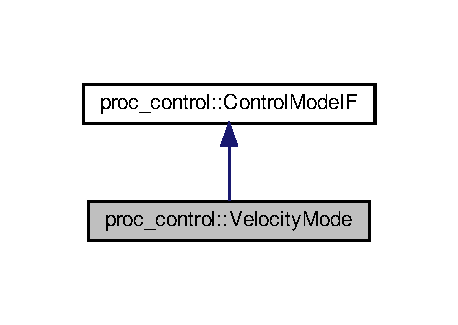
\includegraphics[width=220pt]{classproc__control_1_1_velocity_mode__inherit__graph}
\end{center}
\end{figure}


Collaboration diagram for proc\+\_\+control\+:\+:Velocity\+Mode\+:\nopagebreak
\begin{figure}[H]
\begin{center}
\leavevmode
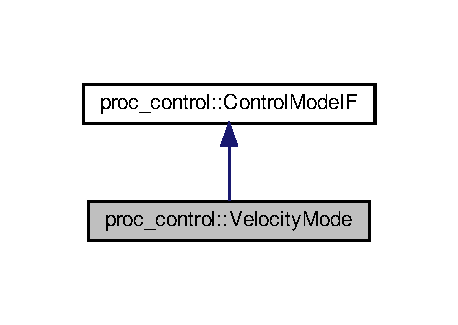
\includegraphics[width=220pt]{classproc__control_1_1_velocity_mode__coll__graph}
\end{center}
\end{figure}
\subsection*{Public Member Functions}
\begin{DoxyCompactItemize}
\item 
\mbox{\Hypertarget{classproc__control_1_1_velocity_mode_ae9b524024246a8ff8404f6673f1e48e5}\label{classproc__control_1_1_velocity_mode_ae9b524024246a8ff8404f6673f1e48e5}} 
{\bfseries Velocity\+Mode} (std\+::shared\+\_\+ptr$<$ \hyperlink{classproc__control_1_1_robot_state}{Robot\+State} $>$ \&robot\+State, std\+::unique\+\_\+ptr$<$ \hyperlink{classproc__control_1_1_controller_i_f}{Controller\+IF} $>$ \&control\+A\+UV)
\item 
\mbox{\Hypertarget{classproc__control_1_1_velocity_mode_aae19dc6c1816b938b4ee3fed99bc59fb}\label{classproc__control_1_1_velocity_mode_aae19dc6c1816b938b4ee3fed99bc59fb}} 
void {\bfseries Process} () override
\item 
\mbox{\Hypertarget{classproc__control_1_1_velocity_mode_a69f4661842a0619df669b73c1c36cbff}\label{classproc__control_1_1_velocity_mode_a69f4661842a0619df669b73c1c36cbff}} 
void {\bfseries Set\+Target} (bool is\+Global, Eigen\+::\+Vector\+Xd \&target\+Pose) override
\item 
\mbox{\Hypertarget{classproc__control_1_1_velocity_mode_aaaa1e4cb5e6ffe0b07db4626068e0b3a}\label{classproc__control_1_1_velocity_mode_aaaa1e4cb5e6ffe0b07db4626068e0b3a}} 
void {\bfseries Set\+Decoupled\+Target} (bool is\+Global, const std\+::vector$<$ bool $>$ \&keep\+Target, Eigen\+::\+Vector\+Xd \&target\+Pose) override
\end{DoxyCompactItemize}


The documentation for this class was generated from the following files\+:\begin{DoxyCompactItemize}
\item 
Mode/Velocity\+Mode.\+h\item 
Mode/Velocity\+Mode.\+cc\end{DoxyCompactItemize}

\chapter{File Documentation}
\hypertarget{_config_manager_8h}{}\section{Config/\+Config\+Manager.h File Reference}
\label{_config_manager_8h}\index{Config/\+Config\+Manager.\+h@{Config/\+Config\+Manager.\+h}}
{\ttfamily \#include $<$string$>$}\newline
{\ttfamily \#include $<$ros/ros.\+h$>$}\newline
{\ttfamily \#include $<$dynamic\+\_\+reconfigure/server.\+h$>$}\newline
{\ttfamily \#include $<$yaml-\/cpp/yaml.\+h$>$}\newline
Include dependency graph for Config\+Manager.\+h\+:\nopagebreak
\begin{figure}[H]
\begin{center}
\leavevmode
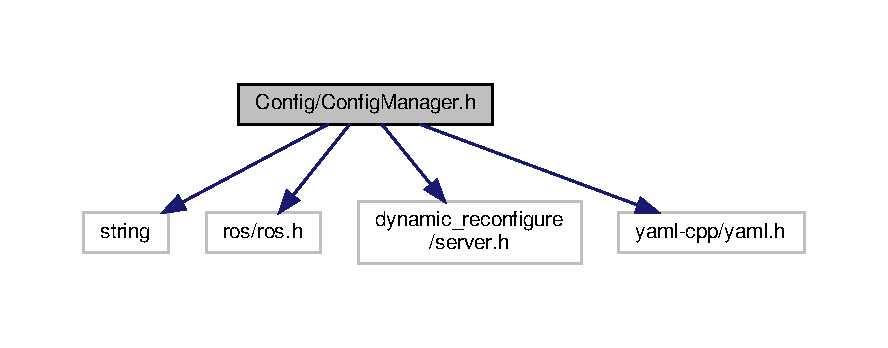
\includegraphics[width=350pt]{_config_manager_8h__incl}
\end{center}
\end{figure}
This graph shows which files directly or indirectly include this file\+:\nopagebreak
\begin{figure}[H]
\begin{center}
\leavevmode
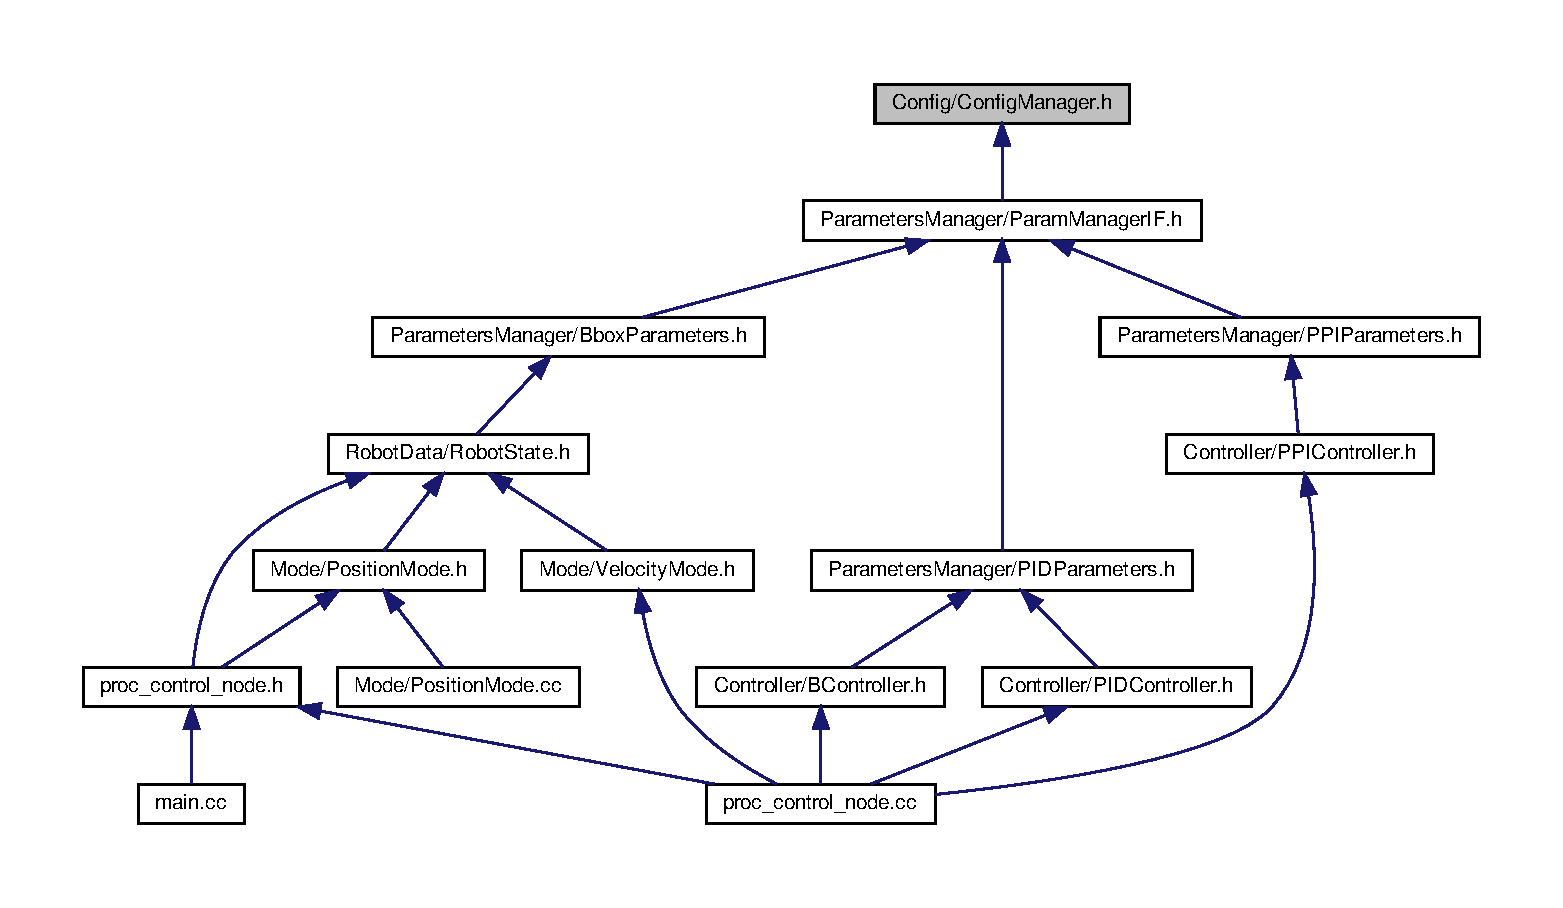
\includegraphics[width=350pt]{_config_manager_8h__dep__incl}
\end{center}
\end{figure}
\subsection*{Classes}
\begin{DoxyCompactItemize}
\item 
class \hyperlink{class_config_manager}{Config\+Manager$<$ T $>$}
\end{DoxyCompactItemize}


\subsection{Detailed Description}
\begin{DoxyAuthor}{Author}
Jeremie St-\/\+Jules \href{mailto:jeremie.st.jules.prevost@gmail.com}{\tt jeremie.\+st.\+jules.\+prevost@gmail.\+com}  Francis Masse \href{mailto:francis.masse05@gmail.com}{\tt francis.\+masse05@gmail.\+com} 
\end{DoxyAuthor}
\begin{DoxyDate}{Date}
10/17/16
\end{DoxyDate}
\begin{DoxyCopyright}{Copyright}
Copyright (c) 2017 S.\+O.\+N.\+I.\+A. A\+UV All rights reserved.
\end{DoxyCopyright}
\hypertarget{_robot_state_8h_LICENSE}{}\subsection{L\+I\+C\+E\+N\+SE}\label{_robot_state_8h_LICENSE}
This file is part of S.\+O.\+N.\+I.\+A. software.

S.\+O.\+N.\+I.\+A. A\+UV software is free software\+: you can redistribute it and/or modify it under the terms of the G\+NU General Public License as published by the Free Software Foundation, either version 3 of the License, or (at your option) any later version.

S.\+O.\+N.\+I.\+A. A\+UV software is distributed in the hope that it will be useful, but W\+I\+T\+H\+O\+UT A\+NY W\+A\+R\+R\+A\+N\+TY; without even the implied warranty of M\+E\+R\+C\+H\+A\+N\+T\+A\+B\+I\+L\+I\+TY or F\+I\+T\+N\+E\+SS F\+OR A P\+A\+R\+T\+I\+C\+U\+L\+AR P\+U\+R\+P\+O\+SE. See the G\+NU General Public License for more details.

You should have received a copy of the G\+NU General Public License along with S.\+O.\+N.\+I.\+A. A\+UV software. If not, see \href{http://www.gnu.org/licenses/}{\tt http\+://www.\+gnu.\+org/licenses/}. 
\hypertarget{_control_input_8cc}{}\section{Control\+Input/\+Control\+Input.cc File Reference}
\label{_control_input_8cc}\index{Control\+Input/\+Control\+Input.\+cc@{Control\+Input/\+Control\+Input.\+cc}}
{\ttfamily \#include \char`\"{}Control\+Input.\+h\char`\"{}}\newline
Include dependency graph for Control\+Input.\+cc\+:\nopagebreak
\begin{figure}[H]
\begin{center}
\leavevmode
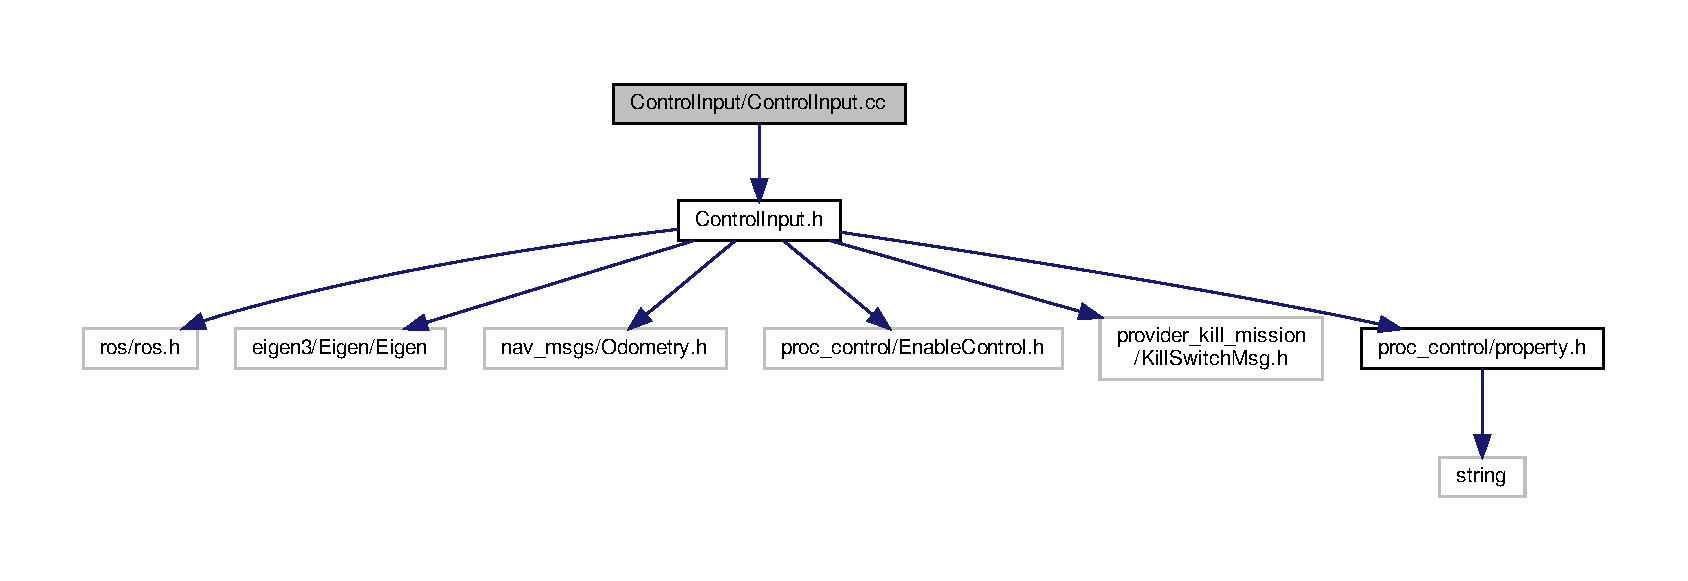
\includegraphics[width=350pt]{_control_input_8cc__incl}
\end{center}
\end{figure}


\subsection{Detailed Description}
\begin{DoxyAuthor}{Author}
Olivier Lavoie \href{mailto:olavoie9507@gmail.com}{\tt olavoie9507@gmail.\+com} 
\end{DoxyAuthor}
\begin{DoxyDate}{Date}
10/21/17
\end{DoxyDate}
\begin{DoxyCopyright}{Copyright}
Copyright (c) 2017 S.\+O.\+N.\+I.\+A. A\+UV All rights reserved.
\end{DoxyCopyright}
\hypertarget{_robot_state_8h_LICENSE}{}\subsection{L\+I\+C\+E\+N\+SE}\label{_robot_state_8h_LICENSE}
This file is part of S.\+O.\+N.\+I.\+A. software.

S.\+O.\+N.\+I.\+A. A\+UV software is free software\+: you can redistribute it and/or modify it under the terms of the G\+NU General Public License as published by the Free Software Foundation, either version 3 of the License, or (at your option) any later version.

S.\+O.\+N.\+I.\+A. A\+UV software is distributed in the hope that it will be useful, but W\+I\+T\+H\+O\+UT A\+NY W\+A\+R\+R\+A\+N\+TY; without even the implied warranty of M\+E\+R\+C\+H\+A\+N\+T\+A\+B\+I\+L\+I\+TY or F\+I\+T\+N\+E\+SS F\+OR A P\+A\+R\+T\+I\+C\+U\+L\+AR P\+U\+R\+P\+O\+SE. See the G\+NU General Public License for more details.

You should have received a copy of the G\+NU General Public License along with S.\+O.\+N.\+I.\+A. A\+UV software. If not, see \href{http://www.gnu.org/licenses/}{\tt http\+://www.\+gnu.\+org/licenses/}. 
\hypertarget{_control_input_8h}{}\section{Control\+Input/\+Control\+Input.h File Reference}
\label{_control_input_8h}\index{Control\+Input/\+Control\+Input.\+h@{Control\+Input/\+Control\+Input.\+h}}
{\ttfamily \#include $<$ros/ros.\+h$>$}\newline
{\ttfamily \#include $<$eigen3/\+Eigen/\+Eigen$>$}\newline
{\ttfamily \#include $<$nav\+\_\+msgs/\+Odometry.\+h$>$}\newline
{\ttfamily \#include \char`\"{}proc\+\_\+control/\+Enable\+Control.\+h\char`\"{}}\newline
{\ttfamily \#include \char`\"{}provider\+\_\+kill\+\_\+mission/\+Kill\+Switch\+Msg.\+h\char`\"{}}\newline
{\ttfamily \#include \char`\"{}proc\+\_\+control/property.\+h\char`\"{}}\newline
Include dependency graph for Control\+Input.\+h\+:\nopagebreak
\begin{figure}[H]
\begin{center}
\leavevmode
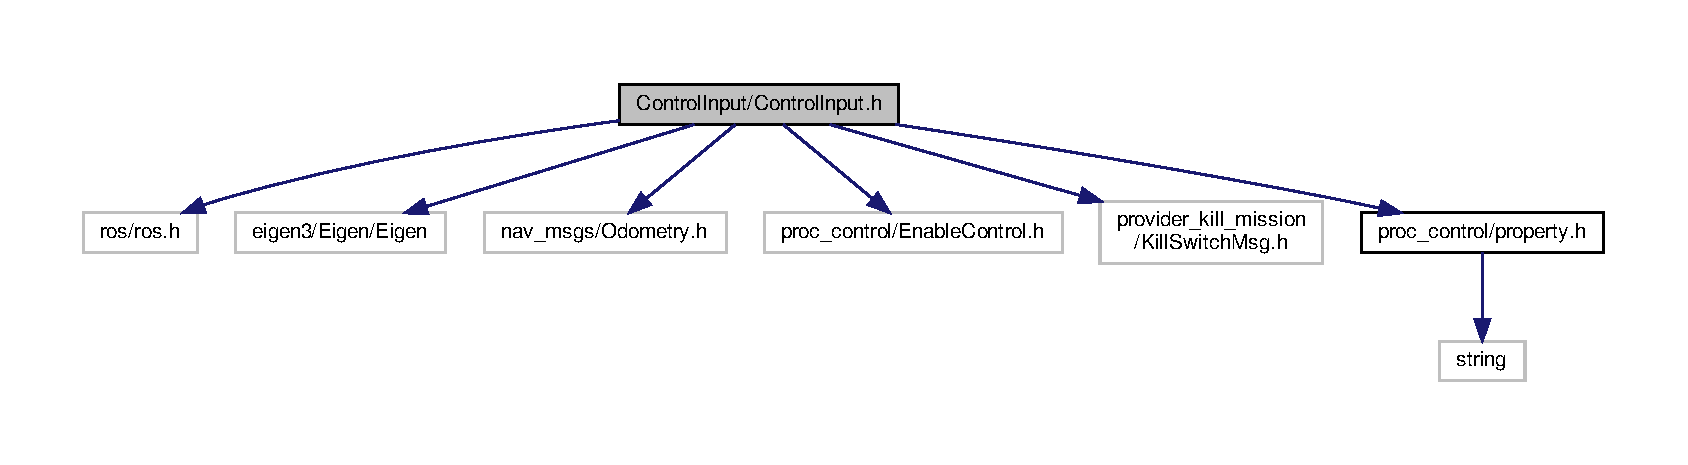
\includegraphics[width=350pt]{_control_input_8h__incl}
\end{center}
\end{figure}
This graph shows which files directly or indirectly include this file\+:\nopagebreak
\begin{figure}[H]
\begin{center}
\leavevmode
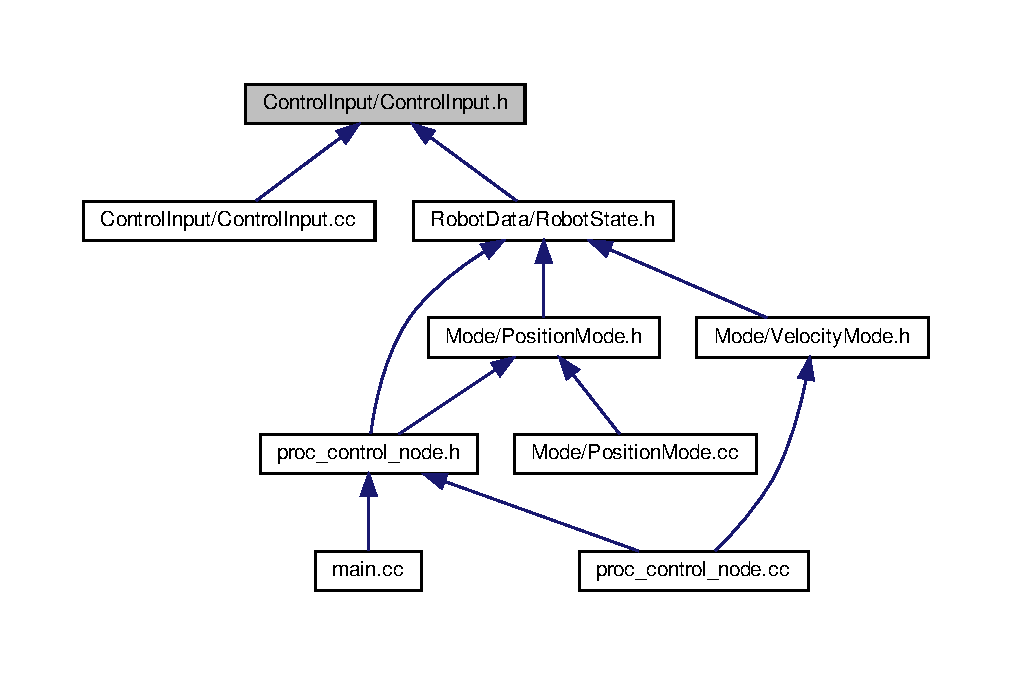
\includegraphics[width=350pt]{_control_input_8h__dep__incl}
\end{center}
\end{figure}
\subsection*{Classes}
\begin{DoxyCompactItemize}
\item 
class \hyperlink{classproc__control_1_1_control_input}{proc\+\_\+control\+::\+Control\+Input}
\end{DoxyCompactItemize}


\subsection{Detailed Description}
\begin{DoxyAuthor}{Author}
Olivier Lavoie \href{mailto:olavoie9507@gmail.com}{\tt olavoie9507@gmail.\+com} 
\end{DoxyAuthor}
\begin{DoxyDate}{Date}
10/21/17
\end{DoxyDate}
\begin{DoxyCopyright}{Copyright}
Copyright (c) 2017 S.\+O.\+N.\+I.\+A. A\+UV All rights reserved.
\end{DoxyCopyright}
\hypertarget{_robot_state_8h_LICENSE}{}\subsection{L\+I\+C\+E\+N\+SE}\label{_robot_state_8h_LICENSE}
This file is part of S.\+O.\+N.\+I.\+A. software.

S.\+O.\+N.\+I.\+A. A\+UV software is free software\+: you can redistribute it and/or modify it under the terms of the G\+NU General Public License as published by the Free Software Foundation, either version 3 of the License, or (at your option) any later version.

S.\+O.\+N.\+I.\+A. A\+UV software is distributed in the hope that it will be useful, but W\+I\+T\+H\+O\+UT A\+NY W\+A\+R\+R\+A\+N\+TY; without even the implied warranty of M\+E\+R\+C\+H\+A\+N\+T\+A\+B\+I\+L\+I\+TY or F\+I\+T\+N\+E\+SS F\+OR A P\+A\+R\+T\+I\+C\+U\+L\+AR P\+U\+R\+P\+O\+SE. See the G\+NU General Public License for more details.

You should have received a copy of the G\+NU General Public License along with S.\+O.\+N.\+I.\+A. A\+UV software. If not, see \href{http://www.gnu.org/licenses/}{\tt http\+://www.\+gnu.\+org/licenses/}. 
\hypertarget{main_8cc}{}\section{main.\+cc File Reference}
\label{main_8cc}\index{main.\+cc@{main.\+cc}}
{\ttfamily \#include $<$ros/ros.\+h$>$}\newline
{\ttfamily \#include \char`\"{}proc\+\_\+control\+\_\+node.\+h\char`\"{}}\newline
Include dependency graph for main.\+cc\+:\nopagebreak
\begin{figure}[H]
\begin{center}
\leavevmode
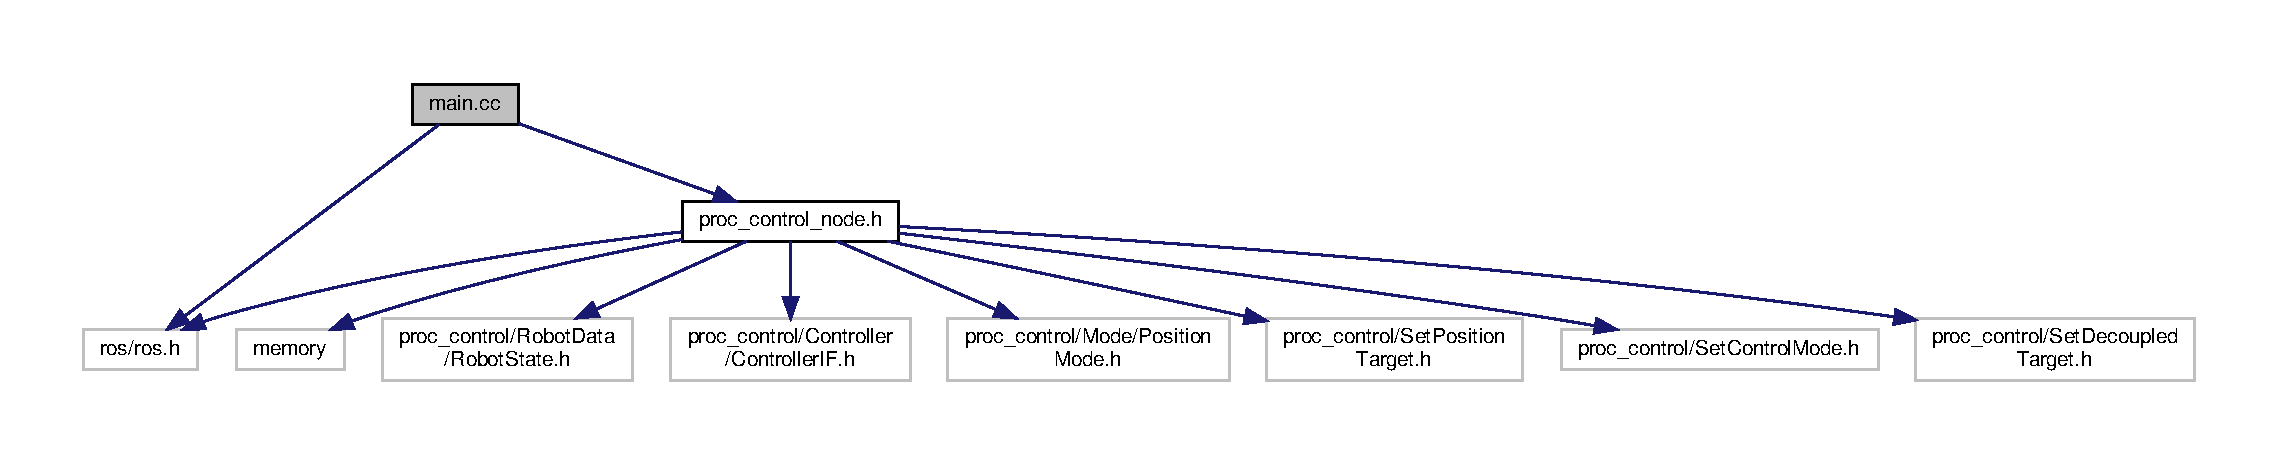
\includegraphics[width=350pt]{main_8cc__incl}
\end{center}
\end{figure}
\subsection*{Functions}
\begin{DoxyCompactItemize}
\item 
\mbox{\Hypertarget{main_8cc_a3c04138a5bfe5d72780bb7e82a18e627}\label{main_8cc_a3c04138a5bfe5d72780bb7e82a18e627}} 
int {\bfseries main} (int argc, char $\ast$$\ast$argv)
\end{DoxyCompactItemize}


\subsection{Detailed Description}
\begin{DoxyAuthor}{Author}
Jeremie St-\/\+Jules-\/\+Prevost \href{mailto:jeremie.st.jules.prevost@gmail.com}{\tt jeremie.\+st.\+jules.\+prevost@gmail.\+com} 
\end{DoxyAuthor}
\begin{DoxyDate}{Date}
24/01/2016
\end{DoxyDate}
\begin{DoxyCopyright}{Copyright}
Copyright (c) 2017 S.\+O.\+N.\+I.\+A. All rights reserved.
\end{DoxyCopyright}
This file contains the main function of proc control.\hypertarget{property_8h_LICENSE}{}\subsection{L\+I\+C\+E\+N\+SE}\label{property_8h_LICENSE}
This file is part of S.\+O.\+N.\+I.\+A. A\+UV software.

S.\+O.\+N.\+I.\+A. A\+UV software is free software\+: you can redistribute it and/or modify it under the terms of the G\+NU General Public License as published by the Free Software Foundation, either version 3 of the License, or (at your option) any later version.

S.\+O.\+N.\+I.\+A. A\+UV software is distributed in the hope that it will be useful, but W\+I\+T\+H\+O\+UT A\+NY W\+A\+R\+R\+A\+N\+TY; without even the implied warranty of M\+E\+R\+C\+H\+A\+N\+T\+A\+B\+I\+L\+I\+TY or F\+I\+T\+N\+E\+SS F\+OR A P\+A\+R\+T\+I\+C\+U\+L\+AR P\+U\+R\+P\+O\+SE. See the G\+NU General Public License for more details.

You should have received a copy of the G\+NU General Public License along with S.\+O.\+N.\+I.\+A. A\+UV software. If not, see \href{http://www.gnu.org/licenses/}{\tt http\+://www.\+gnu.\+org/licenses/}. 
\hypertarget{_control_mode_i_f_8h}{}\section{Mode/\+Control\+Mode\+IF.h File Reference}
\label{_control_mode_i_f_8h}\index{Mode/\+Control\+Mode\+I\+F.\+h@{Mode/\+Control\+Mode\+I\+F.\+h}}
{\ttfamily \#include $<$eigen3/\+Eigen/\+Eigen$>$}\newline
Include dependency graph for Control\+Mode\+I\+F.\+h\+:\nopagebreak
\begin{figure}[H]
\begin{center}
\leavevmode
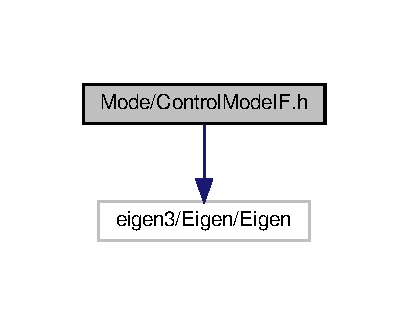
\includegraphics[width=196pt]{_control_mode_i_f_8h__incl}
\end{center}
\end{figure}
This graph shows which files directly or indirectly include this file\+:\nopagebreak
\begin{figure}[H]
\begin{center}
\leavevmode
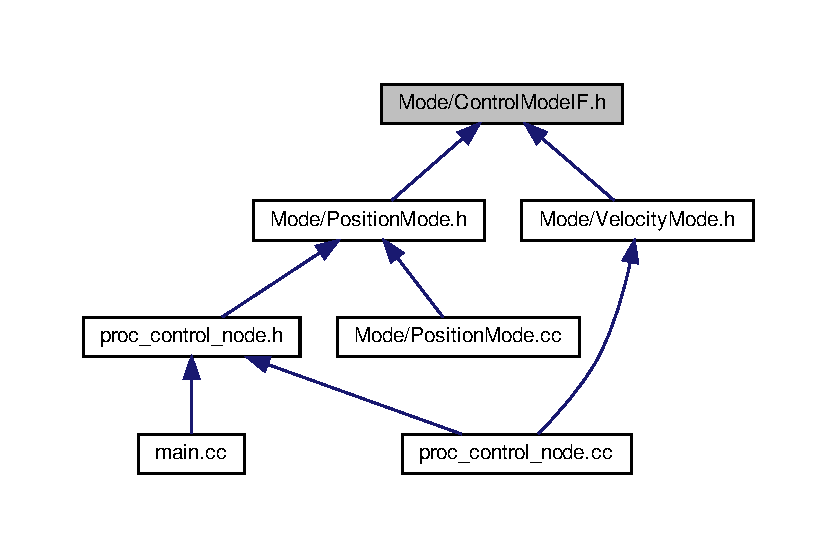
\includegraphics[width=350pt]{_control_mode_i_f_8h__dep__incl}
\end{center}
\end{figure}
\subsection*{Classes}
\begin{DoxyCompactItemize}
\item 
class \hyperlink{classproc__control_1_1_control_mode_i_f}{proc\+\_\+control\+::\+Control\+Mode\+IF}
\end{DoxyCompactItemize}


\subsection{Detailed Description}
\begin{DoxyAuthor}{Author}
Olivier Lavoie \href{mailto:olavoie9507@gmail.com}{\tt olavoie9507@gmail.\+com} 
\end{DoxyAuthor}
\begin{DoxyDate}{Date}
10/21/17
\end{DoxyDate}
\begin{DoxyCopyright}{Copyright}
Copyright (c) 2017 S.\+O.\+N.\+I.\+A. A\+UV All rights reserved.
\end{DoxyCopyright}
\hypertarget{_robot_state_8h_LICENSE}{}\subsection{L\+I\+C\+E\+N\+SE}\label{_robot_state_8h_LICENSE}
This file is part of S.\+O.\+N.\+I.\+A. software.

S.\+O.\+N.\+I.\+A. A\+UV software is free software\+: you can redistribute it and/or modify it under the terms of the G\+NU General Public License as published by the Free Software Foundation, either version 3 of the License, or (at your option) any later version.

S.\+O.\+N.\+I.\+A. A\+UV software is distributed in the hope that it will be useful, but W\+I\+T\+H\+O\+UT A\+NY W\+A\+R\+R\+A\+N\+TY; without even the implied warranty of M\+E\+R\+C\+H\+A\+N\+T\+A\+B\+I\+L\+I\+TY or F\+I\+T\+N\+E\+SS F\+OR A P\+A\+R\+T\+I\+C\+U\+L\+AR P\+U\+R\+P\+O\+SE. See the G\+NU General Public License for more details.

You should have received a copy of the G\+NU General Public License along with S.\+O.\+N.\+I.\+A. A\+UV software. If not, see \href{http://www.gnu.org/licenses/}{\tt http\+://www.\+gnu.\+org/licenses/}. 
\hypertarget{_position_mode_8cc}{}\section{Mode/\+Position\+Mode.cc File Reference}
\label{_position_mode_8cc}\index{Mode/\+Position\+Mode.\+cc@{Mode/\+Position\+Mode.\+cc}}
{\ttfamily \#include $<$control\+\_\+library/toolbox/\+Transformation.\+h$>$}\newline
{\ttfamily \#include \char`\"{}Position\+Mode.\+h\char`\"{}}\newline
Include dependency graph for Position\+Mode.\+cc\+:\nopagebreak
\begin{figure}[H]
\begin{center}
\leavevmode
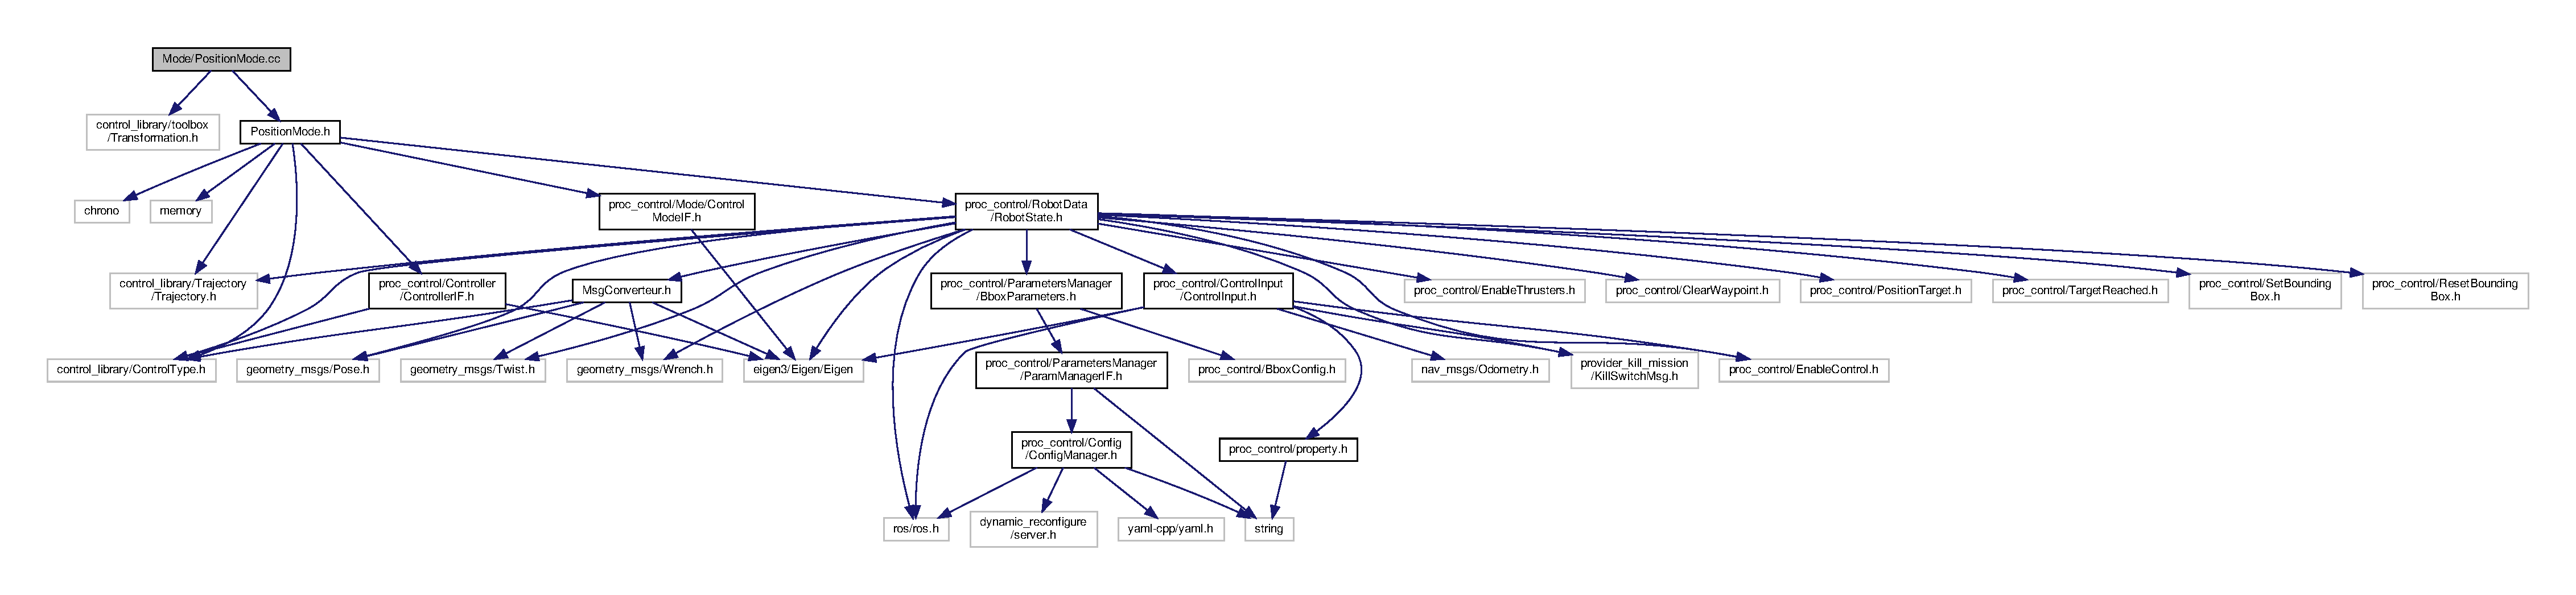
\includegraphics[width=350pt]{_position_mode_8cc__incl}
\end{center}
\end{figure}


\subsection{Detailed Description}
\begin{DoxyAuthor}{Author}
Olivier Lavoie \href{mailto:olavoie9507@gmail.com}{\tt olavoie9507@gmail.\+com} 
\end{DoxyAuthor}
\begin{DoxyDate}{Date}
10/21/17
\end{DoxyDate}
\begin{DoxyCopyright}{Copyright}
Copyright (c) 2017 S.\+O.\+N.\+I.\+A. A\+UV All rights reserved.
\end{DoxyCopyright}
\hypertarget{_robot_state_8h_LICENSE}{}\subsection{L\+I\+C\+E\+N\+SE}\label{_robot_state_8h_LICENSE}
This file is part of S.\+O.\+N.\+I.\+A. software.

S.\+O.\+N.\+I.\+A. A\+UV software is free software\+: you can redistribute it and/or modify it under the terms of the G\+NU General Public License as published by the Free Software Foundation, either version 3 of the License, or (at your option) any later version.

S.\+O.\+N.\+I.\+A. A\+UV software is distributed in the hope that it will be useful, but W\+I\+T\+H\+O\+UT A\+NY W\+A\+R\+R\+A\+N\+TY; without even the implied warranty of M\+E\+R\+C\+H\+A\+N\+T\+A\+B\+I\+L\+I\+TY or F\+I\+T\+N\+E\+SS F\+OR A P\+A\+R\+T\+I\+C\+U\+L\+AR P\+U\+R\+P\+O\+SE. See the G\+NU General Public License for more details.

You should have received a copy of the G\+NU General Public License along with S.\+O.\+N.\+I.\+A. A\+UV software. If not, see \href{http://www.gnu.org/licenses/}{\tt http\+://www.\+gnu.\+org/licenses/}. 
\hypertarget{_position_mode_8h}{}\section{Mode/\+Position\+Mode.h File Reference}
\label{_position_mode_8h}\index{Mode/\+Position\+Mode.\+h@{Mode/\+Position\+Mode.\+h}}
{\ttfamily \#include $<$chrono$>$}\newline
{\ttfamily \#include $<$memory$>$}\newline
{\ttfamily \#include $<$control\+\_\+library/\+Trajectory/\+Trajectory.\+h$>$}\newline
{\ttfamily \#include $<$control\+\_\+library/\+Control\+Type.\+h$>$}\newline
{\ttfamily \#include \char`\"{}proc\+\_\+control/\+Robot\+Data/\+Robot\+State.\+h\char`\"{}}\newline
{\ttfamily \#include \char`\"{}proc\+\_\+control/\+Controller/\+Controller\+I\+F.\+h\char`\"{}}\newline
{\ttfamily \#include \char`\"{}proc\+\_\+control/\+Mode/\+Control\+Mode\+I\+F.\+h\char`\"{}}\newline
Include dependency graph for Position\+Mode.\+h\+:\nopagebreak
\begin{figure}[H]
\begin{center}
\leavevmode
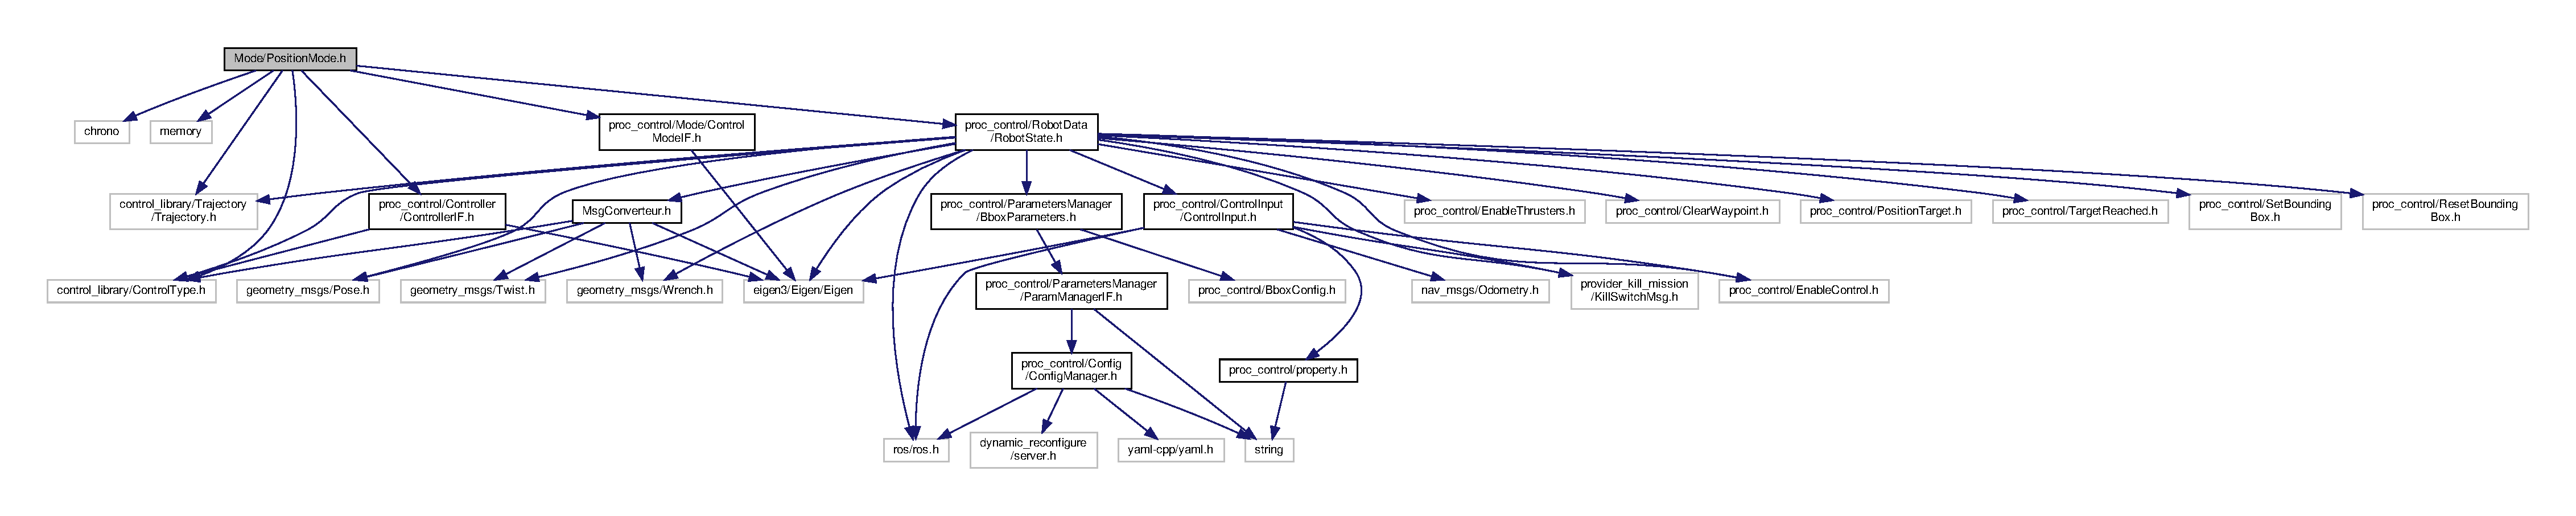
\includegraphics[width=350pt]{_position_mode_8h__incl}
\end{center}
\end{figure}
This graph shows which files directly or indirectly include this file\+:\nopagebreak
\begin{figure}[H]
\begin{center}
\leavevmode
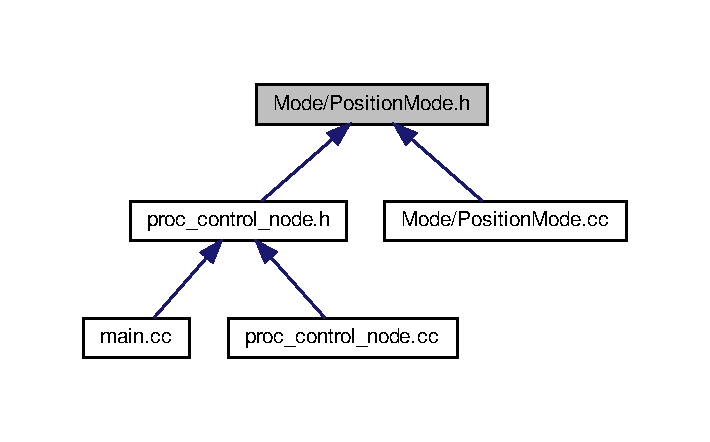
\includegraphics[width=341pt]{_position_mode_8h__dep__incl}
\end{center}
\end{figure}
\subsection*{Classes}
\begin{DoxyCompactItemize}
\item 
class \hyperlink{classproc__control_1_1_position_mode}{proc\+\_\+control\+::\+Position\+Mode}
\end{DoxyCompactItemize}


\subsection{Detailed Description}
\begin{DoxyAuthor}{Author}
Olivier Lavoie \href{mailto:olavoie9507@gmail.com}{\tt olavoie9507@gmail.\+com} 
\end{DoxyAuthor}
\begin{DoxyDate}{Date}
10/21/17
\end{DoxyDate}
\begin{DoxyCopyright}{Copyright}
Copyright (c) 2017 S.\+O.\+N.\+I.\+A. A\+UV All rights reserved.
\end{DoxyCopyright}
\hypertarget{_robot_state_8h_LICENSE}{}\subsection{L\+I\+C\+E\+N\+SE}\label{_robot_state_8h_LICENSE}
This file is part of S.\+O.\+N.\+I.\+A. software.

S.\+O.\+N.\+I.\+A. A\+UV software is free software\+: you can redistribute it and/or modify it under the terms of the G\+NU General Public License as published by the Free Software Foundation, either version 3 of the License, or (at your option) any later version.

S.\+O.\+N.\+I.\+A. A\+UV software is distributed in the hope that it will be useful, but W\+I\+T\+H\+O\+UT A\+NY W\+A\+R\+R\+A\+N\+TY; without even the implied warranty of M\+E\+R\+C\+H\+A\+N\+T\+A\+B\+I\+L\+I\+TY or F\+I\+T\+N\+E\+SS F\+OR A P\+A\+R\+T\+I\+C\+U\+L\+AR P\+U\+R\+P\+O\+SE. See the G\+NU General Public License for more details.

You should have received a copy of the G\+NU General Public License along with S.\+O.\+N.\+I.\+A. A\+UV software. If not, see \href{http://www.gnu.org/licenses/}{\tt http\+://www.\+gnu.\+org/licenses/}. 
\hypertarget{proc__control__node_8cc}{}\section{proc\+\_\+control\+\_\+node.\+cc File Reference}
\label{proc__control__node_8cc}\index{proc\+\_\+control\+\_\+node.\+cc@{proc\+\_\+control\+\_\+node.\+cc}}
{\ttfamily \#include \char`\"{}proc\+\_\+control\+\_\+node.\+h\char`\"{}}\newline
{\ttfamily \#include \char`\"{}proc\+\_\+control/\+Mode/\+Velocity\+Mode.\+h\char`\"{}}\newline
{\ttfamily \#include \char`\"{}proc\+\_\+control/\+Controller/\+P\+I\+D\+Controller.\+h\char`\"{}}\newline
{\ttfamily \#include \char`\"{}proc\+\_\+control/\+Controller/\+P\+P\+I\+Controller.\+h\char`\"{}}\newline
{\ttfamily \#include \char`\"{}proc\+\_\+control/\+Controller/\+B\+Controller.\+h\char`\"{}}\newline
Include dependency graph for proc\+\_\+control\+\_\+node.\+cc\+:\nopagebreak
\begin{figure}[H]
\begin{center}
\leavevmode
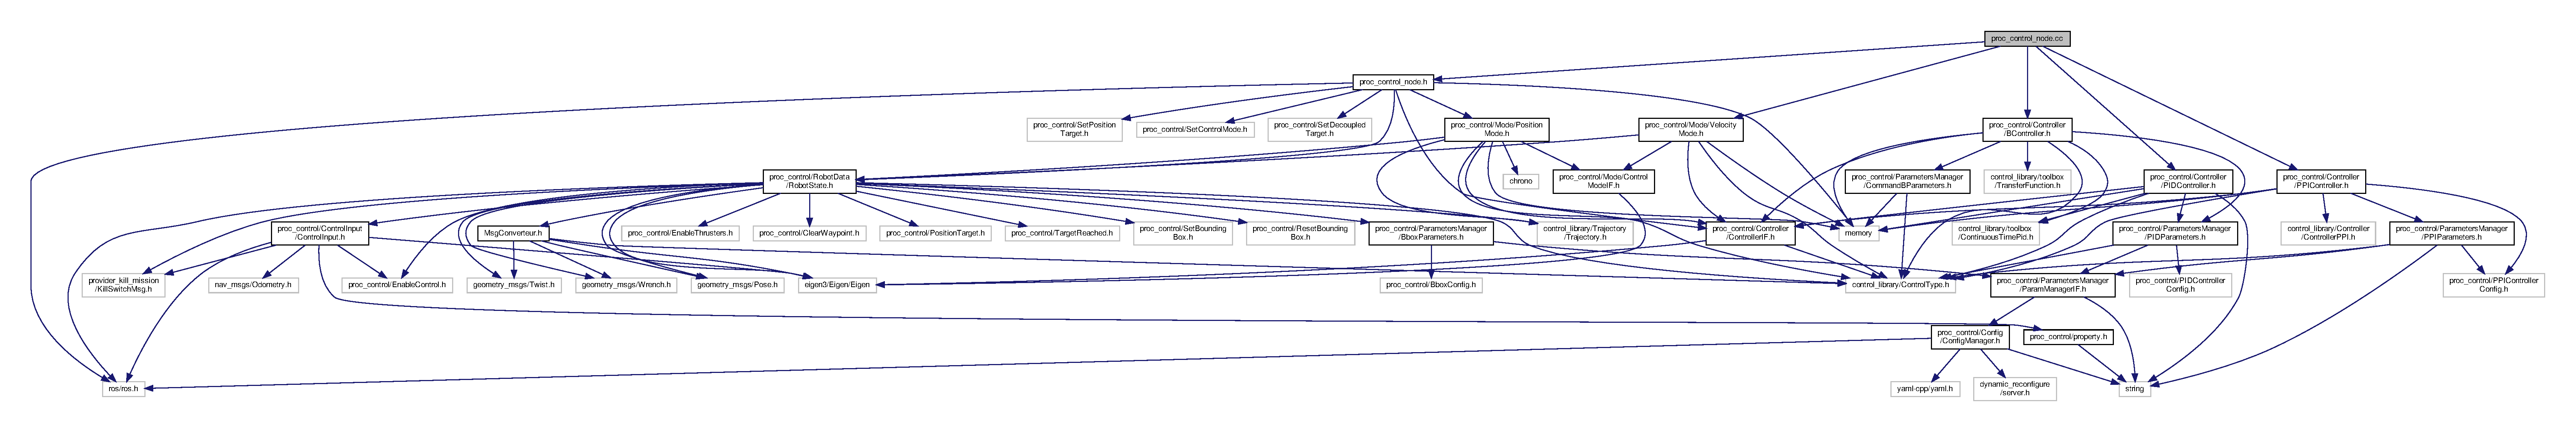
\includegraphics[width=350pt]{proc__control__node_8cc__incl}
\end{center}
\end{figure}


\subsection{Detailed Description}
\begin{DoxyAuthor}{Author}
Olivier Lavoie \href{mailto:olavoie9507@gmail.com}{\tt olavoie9507@gmail.\+com} 
\end{DoxyAuthor}
\begin{DoxyDate}{Date}
10/21/17
\end{DoxyDate}
\begin{DoxyCopyright}{Copyright}
Copyright (c) 2017 S.\+O.\+N.\+I.\+A. A\+UV All rights reserved.
\end{DoxyCopyright}
This file contains the proc control node code.\hypertarget{_robot_state_8h_LICENSE}{}\subsection{L\+I\+C\+E\+N\+SE}\label{_robot_state_8h_LICENSE}
This file is part of S.\+O.\+N.\+I.\+A. software.

S.\+O.\+N.\+I.\+A. A\+UV software is free software\+: you can redistribute it and/or modify it under the terms of the G\+NU General Public License as published by the Free Software Foundation, either version 3 of the License, or (at your option) any later version.

S.\+O.\+N.\+I.\+A. A\+UV software is distributed in the hope that it will be useful, but W\+I\+T\+H\+O\+UT A\+NY W\+A\+R\+R\+A\+N\+TY; without even the implied warranty of M\+E\+R\+C\+H\+A\+N\+T\+A\+B\+I\+L\+I\+TY or F\+I\+T\+N\+E\+SS F\+OR A P\+A\+R\+T\+I\+C\+U\+L\+AR P\+U\+R\+P\+O\+SE. See the G\+NU General Public License for more details.

You should have received a copy of the G\+NU General Public License along with S.\+O.\+N.\+I.\+A. A\+UV software. If not, see \href{http://www.gnu.org/licenses/}{\tt http\+://www.\+gnu.\+org/licenses/}. 
\hypertarget{proc__control__node_8h}{}\section{proc\+\_\+control\+\_\+node.\+h File Reference}
\label{proc__control__node_8h}\index{proc\+\_\+control\+\_\+node.\+h@{proc\+\_\+control\+\_\+node.\+h}}
{\ttfamily \#include $<$ros/ros.\+h$>$}\newline
{\ttfamily \#include $<$memory$>$}\newline
{\ttfamily \#include \char`\"{}proc\+\_\+control/\+Robot\+Data/\+Robot\+State.\+h\char`\"{}}\newline
{\ttfamily \#include \char`\"{}proc\+\_\+control/\+Controller/\+Controller\+I\+F.\+h\char`\"{}}\newline
{\ttfamily \#include \char`\"{}proc\+\_\+control/\+Mode/\+Position\+Mode.\+h\char`\"{}}\newline
{\ttfamily \#include \char`\"{}proc\+\_\+control/\+Set\+Position\+Target.\+h\char`\"{}}\newline
{\ttfamily \#include \char`\"{}proc\+\_\+control/\+Set\+Control\+Mode.\+h\char`\"{}}\newline
{\ttfamily \#include \char`\"{}proc\+\_\+control/\+Set\+Decoupled\+Target.\+h\char`\"{}}\newline
Include dependency graph for proc\+\_\+control\+\_\+node.\+h\+:\nopagebreak
\begin{figure}[H]
\begin{center}
\leavevmode
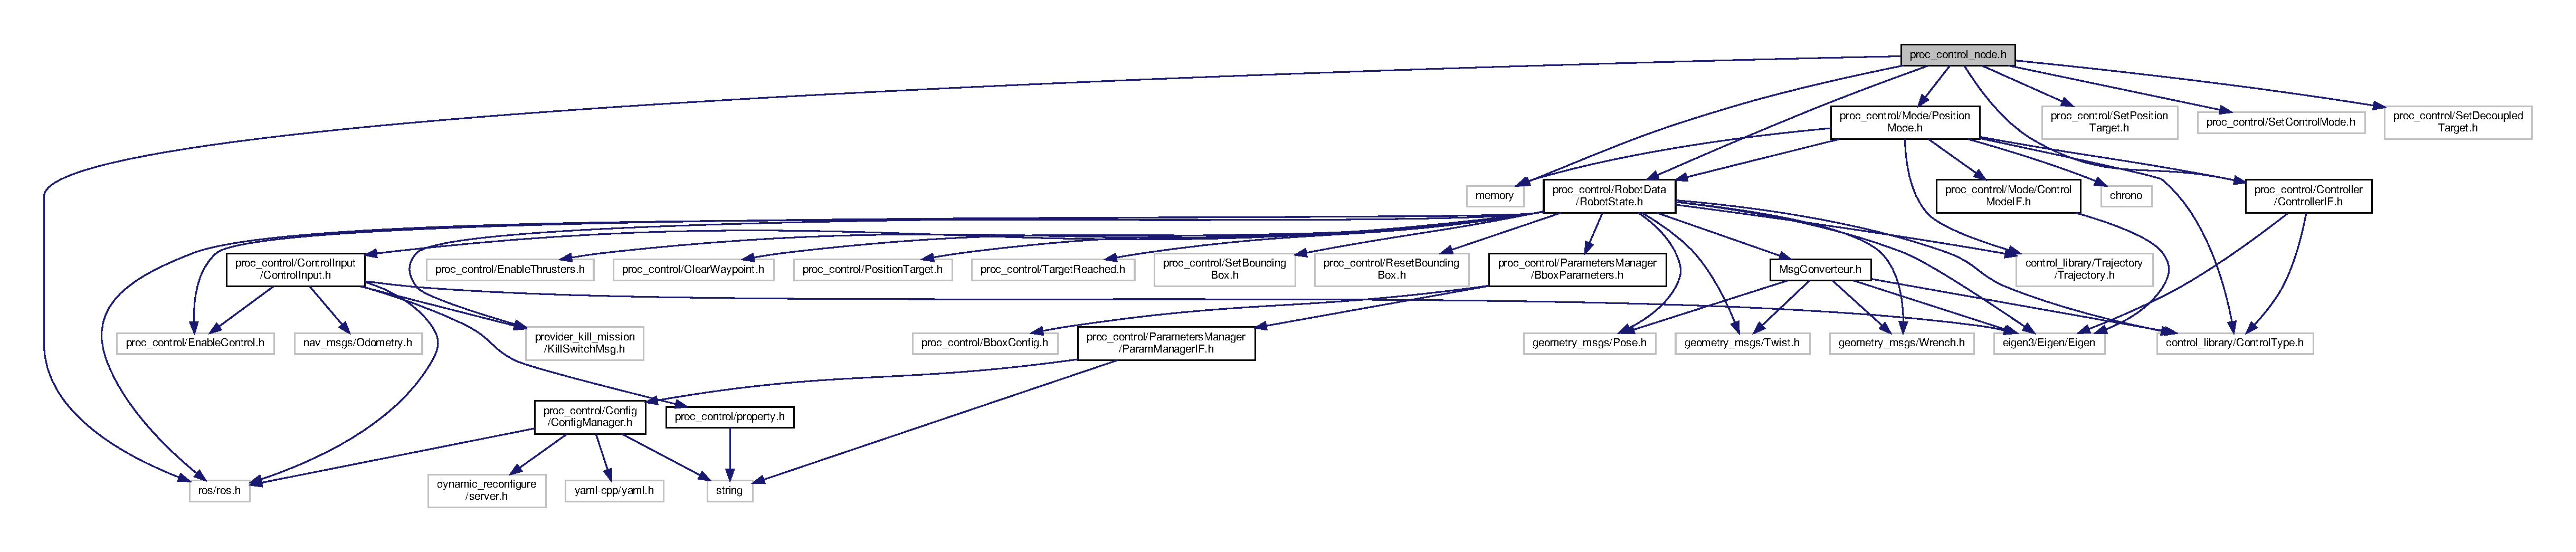
\includegraphics[width=350pt]{proc__control__node_8h__incl}
\end{center}
\end{figure}
This graph shows which files directly or indirectly include this file\+:\nopagebreak
\begin{figure}[H]
\begin{center}
\leavevmode
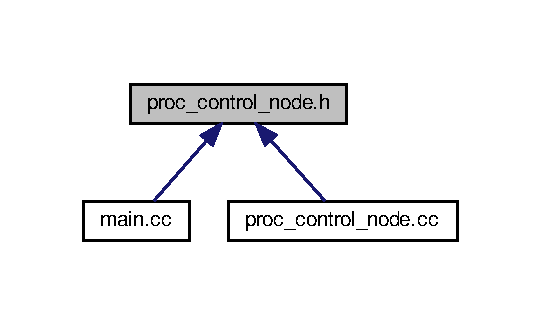
\includegraphics[width=260pt]{proc__control__node_8h__dep__incl}
\end{center}
\end{figure}
\subsection*{Classes}
\begin{DoxyCompactItemize}
\item 
class \hyperlink{classproc__control_1_1_proc_control_node}{proc\+\_\+control\+::\+Proc\+Control\+Node}
\end{DoxyCompactItemize}


\subsection{Detailed Description}
\begin{DoxyAuthor}{Author}
Olivier Lavoie \href{mailto:olavoie9507@gmail.com}{\tt olavoie9507@gmail.\+com} 
\end{DoxyAuthor}
\begin{DoxyDate}{Date}
10/21/17
\end{DoxyDate}
\begin{DoxyCopyright}{Copyright}
Copyright (c) 2017 S.\+O.\+N.\+I.\+A. A\+UV All rights reserved.
\end{DoxyCopyright}
\hypertarget{property_8h_LICENSE}{}\subsection{L\+I\+C\+E\+N\+SE}\label{property_8h_LICENSE}
This file is part of S.\+O.\+N.\+I.\+A. software.

S.\+O.\+N.\+I.\+A. A\+UV software is free software\+: you can redistribute it and/or modify it under the terms of the G\+NU General Public License as published by the Free Software Foundation, either version 3 of the License, or (at your option) any later version.

S.\+O.\+N.\+I.\+A. A\+UV software is distributed in the hope that it will be useful, but W\+I\+T\+H\+O\+UT A\+NY W\+A\+R\+R\+A\+N\+TY; without even the implied warranty of M\+E\+R\+C\+H\+A\+N\+T\+A\+B\+I\+L\+I\+TY or F\+I\+T\+N\+E\+SS F\+OR A P\+A\+R\+T\+I\+C\+U\+L\+AR P\+U\+R\+P\+O\+SE. See the G\+NU General Public License for more details.

You should have received a copy of the G\+NU General Public License along with S.\+O.\+N.\+I.\+A. A\+UV software. If not, see \href{http://www.gnu.org/licenses/}{\tt http\+://www.\+gnu.\+org/licenses/}. 
\hypertarget{property_8h}{}\section{property.\+h File Reference}
\label{property_8h}\index{property.\+h@{property.\+h}}
{\ttfamily \#include $<$string$>$}\newline
Include dependency graph for property.\+h\+:\nopagebreak
\begin{figure}[H]
\begin{center}
\leavevmode
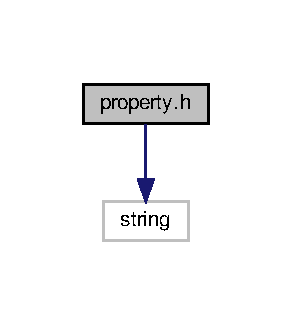
\includegraphics[width=140pt]{property_8h__incl}
\end{center}
\end{figure}
This graph shows which files directly or indirectly include this file\+:\nopagebreak
\begin{figure}[H]
\begin{center}
\leavevmode
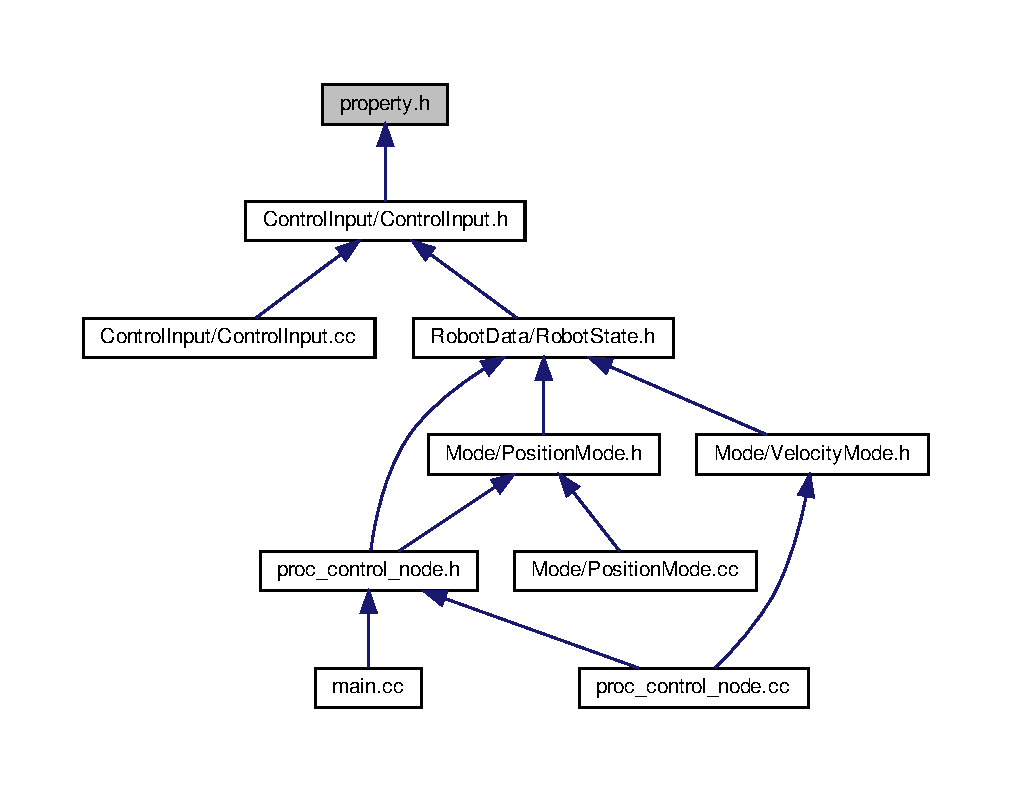
\includegraphics[width=350pt]{property_8h__dep__incl}
\end{center}
\end{figure}
\subsection*{Variables}
\begin{DoxyCompactItemize}
\item 
\mbox{\Hypertarget{property_8h_a68cf5fea512727a0fbb62b558806c3c1}\label{property_8h_a68cf5fea512727a0fbb62b558806c3c1}} 
const std\+::string {\bfseries k\+Node\+Name} = \char`\"{}/proc\+\_\+control/\char`\"{}
\item 
\mbox{\Hypertarget{property_8h_af953190bfe09191220bd3575b48c3ead}\label{property_8h_af953190bfe09191220bd3575b48c3ead}} 
const std\+::string {\bfseries k\+Project\+Folder\+Path} = std\+::getenv(\char`\"{}R\+O\+S\+\_\+\+S\+O\+N\+I\+A\+\_\+\+WS\char`\"{})
\item 
\mbox{\Hypertarget{property_8h_ad49938ab28b6f7e5f9c35f110fbb5661}\label{property_8h_ad49938ab28b6f7e5f9c35f110fbb5661}} 
const std\+::string {\bfseries k\+Project\+Path} = k\+Project\+Folder\+Path + \char`\"{}/src\char`\"{} + k\+Node\+Name
\item 
\mbox{\Hypertarget{property_8h_afb7b8f6b780fc7e694f6d3e2518bd150}\label{property_8h_afb7b8f6b780fc7e694f6d3e2518bd150}} 
const std\+::string {\bfseries k\+Config\+Path} = k\+Project\+Path + \char`\"{}config/\char`\"{}
\item 
\mbox{\Hypertarget{property_8h_a7adb0ba85632ab52d9a045eb226cba83}\label{property_8h_a7adb0ba85632ab52d9a045eb226cba83}} 
const std\+::string {\bfseries k\+Config\+Ext} = \char`\"{}.yaml\char`\"{}
\item 
\mbox{\Hypertarget{property_8h_ab2ce89e06bf93c79ecbf61b36b4658d3}\label{property_8h_ab2ce89e06bf93c79ecbf61b36b4658d3}} 
const size\+\_\+t {\bfseries X} = 0
\item 
\mbox{\Hypertarget{property_8h_a112d438ef5f2ea76a8a154cee2f309e9}\label{property_8h_a112d438ef5f2ea76a8a154cee2f309e9}} 
const size\+\_\+t {\bfseries Y} = 1
\item 
\mbox{\Hypertarget{property_8h_aef46543dd4e4165b2e7decb928628bde}\label{property_8h_aef46543dd4e4165b2e7decb928628bde}} 
const size\+\_\+t {\bfseries Z} = 2
\item 
\mbox{\Hypertarget{property_8h_a0b30a8d3df3bec8de793cabe32d84e87}\label{property_8h_a0b30a8d3df3bec8de793cabe32d84e87}} 
const size\+\_\+t {\bfseries R\+O\+LL} = 3
\item 
\mbox{\Hypertarget{property_8h_a33dde2ba01238d9f9148eddbc532bf05}\label{property_8h_a33dde2ba01238d9f9148eddbc532bf05}} 
const size\+\_\+t {\bfseries P\+I\+T\+CH} = 4
\item 
\mbox{\Hypertarget{property_8h_ad04db1cb686a759abcee818e81f2852e}\label{property_8h_ad04db1cb686a759abcee818e81f2852e}} 
const size\+\_\+t {\bfseries Y\+AW} = 5
\end{DoxyCompactItemize}


\subsection{Detailed Description}
\begin{DoxyAuthor}{Author}
Jeremie St-\/\+Jules-\/\+Prevost \href{mailto:jeremie.st.jules.prevost@gmail.com}{\tt jeremie.\+st.\+jules.\+prevost@gmail.\+com} 
\end{DoxyAuthor}
\begin{DoxyDate}{Date}
2016
\end{DoxyDate}
\begin{DoxyCopyright}{Copyright}
Copyright (c) 2017 S.\+O.\+N.\+I.\+A. All rights reserved.
\end{DoxyCopyright}
This file contains all the constants properties for the proc control.\hypertarget{_robot_state_8h_LICENSE}{}\subsection{L\+I\+C\+E\+N\+SE}\label{_robot_state_8h_LICENSE}
This file is part of S.\+O.\+N.\+I.\+A. software.

S.\+O.\+N.\+I.\+A. A\+UV software is free software\+: you can redistribute it and/or modify it under the terms of the G\+NU General Public License as published by the Free Software Foundation, either version 3 of the License, or (at your option) any later version.

S.\+O.\+N.\+I.\+A. A\+UV software is distributed in the hope that it will be useful, but W\+I\+T\+H\+O\+UT A\+NY W\+A\+R\+R\+A\+N\+TY; without even the implied warranty of M\+E\+R\+C\+H\+A\+N\+T\+A\+B\+I\+L\+I\+TY or F\+I\+T\+N\+E\+SS F\+OR A P\+A\+R\+T\+I\+C\+U\+L\+AR P\+U\+R\+P\+O\+SE. See the G\+NU General Public License for more details.

You should have received a copy of the G\+NU General Public License along with S.\+O.\+N.\+I.\+A. A\+UV software. If not, see \href{http://www.gnu.org/licenses/}{\tt http\+://www.\+gnu.\+org/licenses/}. 
\hypertarget{_robot_state_8h}{}\section{Robot\+Data/\+Robot\+State.h File Reference}
\label{_robot_state_8h}\index{Robot\+Data/\+Robot\+State.\+h@{Robot\+Data/\+Robot\+State.\+h}}
{\ttfamily \#include $<$ros/ros.\+h$>$}\newline
{\ttfamily \#include $<$geometry\+\_\+msgs/\+Pose.\+h$>$}\newline
{\ttfamily \#include $<$geometry\+\_\+msgs/\+Twist.\+h$>$}\newline
{\ttfamily \#include $<$geometry\+\_\+msgs/\+Wrench.\+h$>$}\newline
{\ttfamily \#include $<$eigen3/\+Eigen/\+Eigen$>$}\newline
{\ttfamily \#include $<$control\+\_\+library/\+Trajectory/\+Trajectory.\+h$>$}\newline
{\ttfamily \#include $<$control\+\_\+library/\+Control\+Type.\+h$>$}\newline
{\ttfamily \#include \char`\"{}provider\+\_\+kill\+\_\+mission/\+Kill\+Switch\+Msg.\+h\char`\"{}}\newline
{\ttfamily \#include \char`\"{}Msg\+Converteur.\+h\char`\"{}}\newline
{\ttfamily \#include \char`\"{}proc\+\_\+control/\+Control\+Input/\+Control\+Input.\+h\char`\"{}}\newline
{\ttfamily \#include \char`\"{}proc\+\_\+control/\+Enable\+Control.\+h\char`\"{}}\newline
{\ttfamily \#include \char`\"{}proc\+\_\+control/\+Enable\+Thrusters.\+h\char`\"{}}\newline
{\ttfamily \#include \char`\"{}proc\+\_\+control/\+Clear\+Waypoint.\+h\char`\"{}}\newline
{\ttfamily \#include \char`\"{}proc\+\_\+control/\+Position\+Target.\+h\char`\"{}}\newline
{\ttfamily \#include \char`\"{}proc\+\_\+control/\+Target\+Reached.\+h\char`\"{}}\newline
{\ttfamily \#include \char`\"{}proc\+\_\+control/\+Set\+Bounding\+Box.\+h\char`\"{}}\newline
{\ttfamily \#include \char`\"{}proc\+\_\+control/\+Reset\+Bounding\+Box.\+h\char`\"{}}\newline
{\ttfamily \#include \char`\"{}proc\+\_\+control/\+Parameters\+Manager/\+Bbox\+Parameters.\+h\char`\"{}}\newline
Include dependency graph for Robot\+State.\+h\+:\nopagebreak
\begin{figure}[H]
\begin{center}
\leavevmode
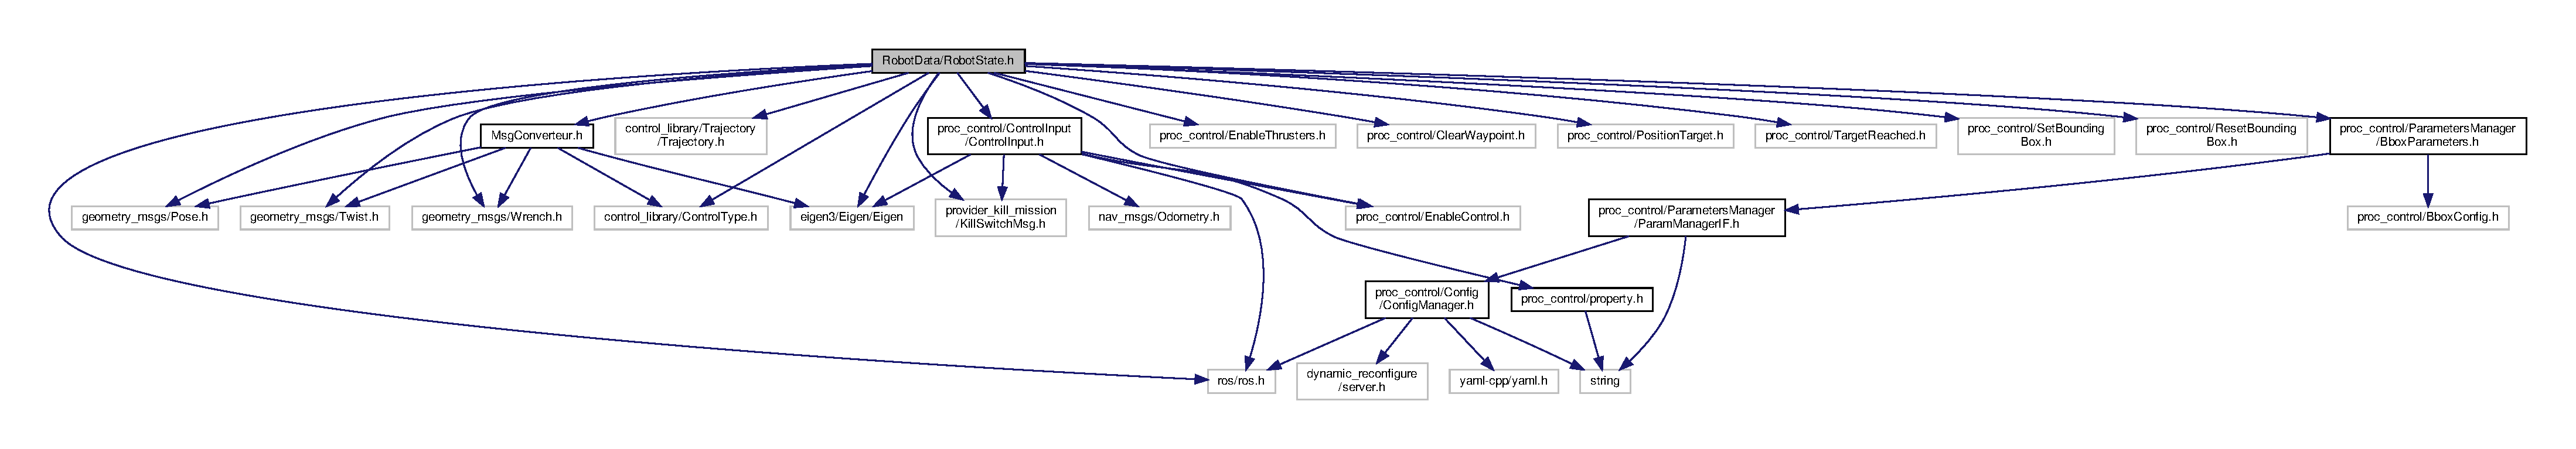
\includegraphics[width=350pt]{_robot_state_8h__incl}
\end{center}
\end{figure}
This graph shows which files directly or indirectly include this file\+:\nopagebreak
\begin{figure}[H]
\begin{center}
\leavevmode
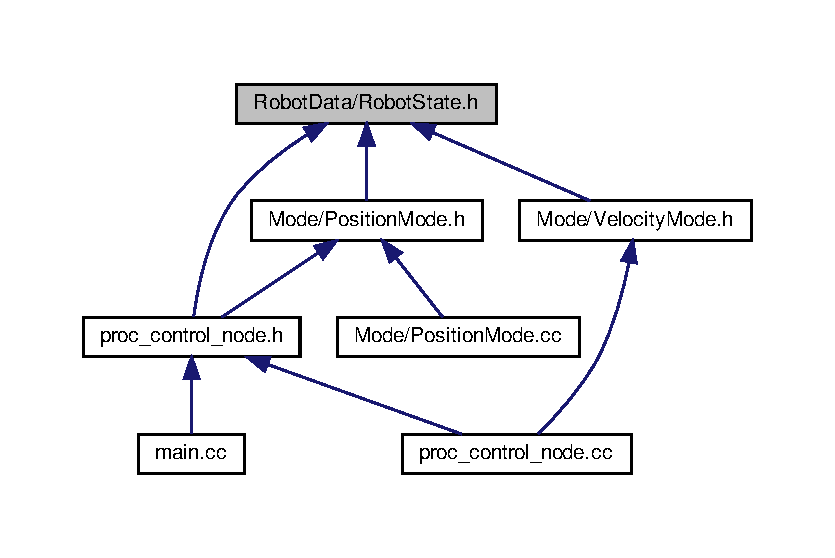
\includegraphics[width=350pt]{_robot_state_8h__dep__incl}
\end{center}
\end{figure}
\subsection*{Classes}
\begin{DoxyCompactItemize}
\item 
class \hyperlink{classproc__control_1_1_robot_state}{proc\+\_\+control\+::\+Robot\+State}
\end{DoxyCompactItemize}
\subsection*{Variables}
\begin{DoxyCompactItemize}
\item 
\mbox{\Hypertarget{_robot_state_8h_a7ee3f522cb3fa1e69eafa9e907cf4a3a}\label{_robot_state_8h_a7ee3f522cb3fa1e69eafa9e907cf4a3a}} 
const double {\bfseries D\+E\+G\+R\+E\+E\+\_\+\+T\+O\+\_\+\+R\+AD} = M\+\_\+\+PI / 180.\+0
\item 
\mbox{\Hypertarget{_robot_state_8h_ae09fdb99d7b35396f160c9c4e633aadc}\label{_robot_state_8h_ae09fdb99d7b35396f160c9c4e633aadc}} 
const double {\bfseries R\+A\+D\+\_\+\+T\+O\+\_\+\+D\+E\+G\+R\+EE} = 180.\+0 / M\+\_\+\+PI
\end{DoxyCompactItemize}


\subsection{Detailed Description}
\begin{DoxyAuthor}{Author}
Olivier Lavoie \href{mailto:olavoie9507@gmail.com}{\tt olavoie9507@gmail.\+com} 
\end{DoxyAuthor}
\begin{DoxyDate}{Date}
10/21/17
\end{DoxyDate}
\begin{DoxyCopyright}{Copyright}
Copyright (c) 2017 S.\+O.\+N.\+I.\+A. A\+UV All rights reserved.
\end{DoxyCopyright}
\hypertarget{_robot_state_8h_LICENSE}{}\subsection{L\+I\+C\+E\+N\+SE}\label{_robot_state_8h_LICENSE}
This file is part of S.\+O.\+N.\+I.\+A. software.

S.\+O.\+N.\+I.\+A. A\+UV software is free software\+: you can redistribute it and/or modify it under the terms of the G\+NU General Public License as published by the Free Software Foundation, either version 3 of the License, or (at your option) any later version.

S.\+O.\+N.\+I.\+A. A\+UV software is distributed in the hope that it will be useful, but W\+I\+T\+H\+O\+UT A\+NY W\+A\+R\+R\+A\+N\+TY; without even the implied warranty of M\+E\+R\+C\+H\+A\+N\+T\+A\+B\+I\+L\+I\+TY or F\+I\+T\+N\+E\+SS F\+OR A P\+A\+R\+T\+I\+C\+U\+L\+AR P\+U\+R\+P\+O\+SE. See the G\+NU General Public License for more details.

You should have received a copy of the G\+NU General Public License along with S.\+O.\+N.\+I.\+A. A\+UV software. If not, see \href{http://www.gnu.org/licenses/}{\tt http\+://www.\+gnu.\+org/licenses/}. 
%--- End generated contents ---

% Index
\backmatter
\newpage
\phantomsection
\clearemptydoublepage
\addcontentsline{toc}{chapter}{Index}
\printindex

\end{document}
